\RequirePackage[l2tabu, orthodox]{nag}

\documentclass[10pt]{scrartcl}
% \documentclass[10pt]{article}
\usepackage[T1]{fontenc}
\usepackage{amsmath,amsfonts,amssymb}
\usepackage{mathtools}
\usepackage{color,soul}
\usepackage[margin=2cm]{geometry}
\usepackage{enumerate}
\usepackage{graphicx}
\usepackage[colorlinks=true,urlcolor=blue]{hyperref}
\usepackage{floatrow}
\usepackage{deluxetable}
\usepackage{verbatim}
\usepackage{fancyvrb}
\usepackage{listings}
\usepackage{calc}
\usepackage[font=small]{caption}
\usepackage[font=scriptsize]{subcaption}
\usepackage[activate={true,nocompatibility},final,tracking=true,kerning=true,spacing=true,factor=1100,stretch=10,shrink=10]{microtype}
\SetTracking{encoding={*}, shape=sc}{40}

\floatsetup{ 
  heightadjust=object,
  valign=t
}

\definecolor{Light}{gray}{.90}
\sethlcolor{Light}


\lstset{%
language=IDL,                   % choose the language of the code
basicstyle=\footnotesize\sffamily,%\ttfamily\footnotesize,       % the size of the fonts that are used for the code
numbers=left,                   % where to put the line-numbers
numberstyle=\footnotesize,      % the size of the fonts that are used for the line-numbers
stepnumber=1,                   % the step between two line-numbers. If it is 1 each line will be numbered
numbersep=5pt,                  % how far the line-numbers are from the code
showspaces=false,               % show spaces adding particular underscores
showstringspaces=false,         % underline spaces within strings
showtabs=false,                 % show tabs within strings adding particular underscores
% frame=single,                   % adds a frame around the code
backgroundcolor=\color{Light},
columns=flexible,
tabsize=2,                      % sets default tabsize to 2 spaces
captionpos=b,                   % sets the caption-position to bottom
breaklines=true,                % sets automatic line breaking
breakatwhitespace=false,        % sets if automatic breaks should only happen at whitespace
escapeinside={\%*}{*)}          % if you want to add a comment within your code
}

\title{Final Documentation Draft}
\author{Jeren Suzuki}
\date{Last Edited \today}

\begin{document}

\maketitle
\pagenumbering{Roman}
\tableofcontents
\clearpage
\pagenumbering{arabic}

\section{Introduction} % (fold)
\label{sec:introduction}
Starting with an image of at most three suns on a fiducial grid, we find their centers and relative position to fiducials (which provide a physical distance calibration). With a 1296 x 966 image with three suns, the program from start to finish takes approximately .15 seconds.
% section introduction (end)

\section{Introduction cont.} % (fold)
\label{sec:intro_cont}
% This outline of steps aims to lay out the basic form we Not sure how in-depth to make the list so I'll just mark it for later.

%%%%%%%%%%%%%%%%%%%%%%%%%%%%%%%%%%%%%%%%%%%%%%%%%%%%%%%%%%%%%%%%%%
%
%
%
%
%
%%%%%%%%%%%%%%%%%%%%%%%%%%%%%%%%%%%%%%%%%%%%%%%%%%%%%%%%%%%%%%%%%%
Code steps:

\begin{enumerate}
    \item Load Image
    \item Load parameters from pblock.txt
    \item Sort image and cut off top .1\% of pixels (top 1\% was actually too much)
    \item Smooth, take deriv, smooth again, take deriv again of sorted array, find peaks that correspond to where the values of different solar regions change. These peaks are used to threshold different solar regions.
    \item Mask image above thresholds to find centers of every shape (sometimes it's not a circle)
    \item If the centroid of the shape is within a certain distance to the image edge, mark as partial and cease further analysis
    \item Crop remaining whole suns
    \item Extract 5 strips around centroid for both X and Y direction
    \item Extract a pair of limb strips for each whole strip
    \item Applt linear fit to limb strips
    \item Use new threshold-crossing positions of fit to calculate chord lengths
    \item Average midpoints of chords to find limb-fitted centers
    \item Analyze the cropped image for fiducials
    \item Using the fiducial positions, compare solar positions to a position defined by the physical setup.
\end{enumerate}


\begin{figure}[!ht]
    \centering
    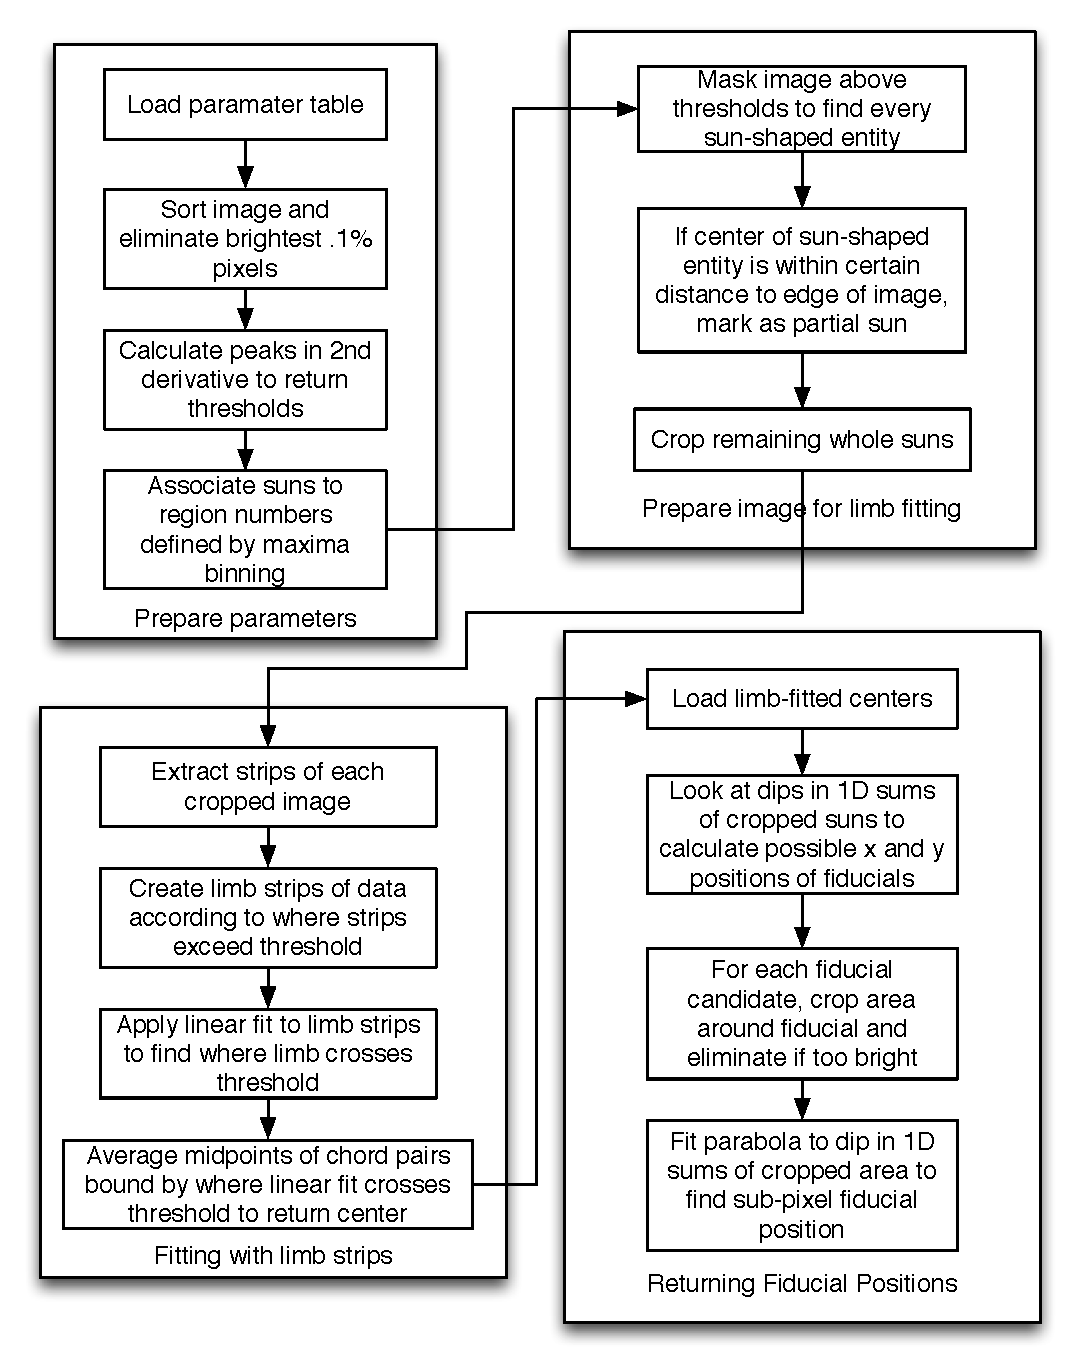
\includegraphics[width=.9\textwidth]{../plots_tables_images/new_alphaflowchart.eps}    
    \caption{}
    \label{flowchart}
\end{figure}


\begin{deluxetable}{cllllllll}
    \tablecaption{Final data structure of solar region}
    \tablecolumns{4}
    \tabletypesize{\scriptsize}
    \tablewidth{0pt}
    \tablehead{ 
      \colhead{Name} %
    & \colhead{Type} %
    & \colhead{Value} %
    & \colhead{Notes}
    }
    \startdata
    \hline
    XPOS
    & FLOAT
    & 210.522
    & Rough calculation using a simple masking method\\
    %
    YPOS
    & FLOAT
    & 166.702
    & ''\\
    %
    REG
    & INT
    & 1
    & Region ID \#: 1 is 100\%, 2 is 50\%, 3 is 25\%\\
    %
    THRESH
    & FLOAT
    & 106.000
    & Threshold calculated from sorting array and taking derivatives.\\ & & & Used in both finding rough X-Y center as well as the\\ & & & threshold for limb-fitting.\\
    %
    PARTIAL
    & FLOAT
    & 0.
    & Flag that determines if the solar region is cut off on the edge or not.\\ & & & 0 means that it is not cut off \\
    %
    XSTRIPS
    & STRUCTURE
    & -> WHOLEXSTRIPS Array[5]
    & Strucutre containing the strips of whole solar data\\ & & & bound by a cropped region chosen by XPOS and YPOS\\
    %
    YSTRIPS
    & STRUCTURE
    & -> WHOLEYSTRIPS Array[5]
    & ''\\
    %
    LIMBXSTRIPS
    & STRUCTURE
    & -> LIMBXSTRIPS Array[5]
    & LIMBSTRIPS contains a pair of arrays, ENDPOINTS and \\ & & & STARTPOINTS that mark the limbs of each strip of data from \\ & & & X/YSTRIPS\\
    %
    LIMBYSTRIPS
    & STRUCTURE
    & -> LIMBYSTRIPS Array[5]
    & ''\\
    %
    LIMBXPOS
    & FLOAT
    & 210.710
    & Center calculated from LIMBXSTRIPS\\
    %
    LIMBYPOS
    & FLOAT
    & 167.172
    & ''\\
    %
    NPIX
    & FLOAT
    & 26680.0
    & Number of pixels above threshold
    \enddata
\label{structtable}
\end{deluxetable}

This is the form of the fiducial structure containing the positions and sub-pixel positions of fiducials for each solar region.
\begin{lstlisting}
>> help,*(bbb[0])
** Structure <260a348>, 2 tags, length=180, data length=178, refs=1:
   REG             INT              1
   FIDARR          STRUCT    -> FIDPOS Array[11]
>> help,(*(bbb[0])).fidarr,/str
** Structure FIDPOS, 4 tags, length=16, data length=16:
   X               FLOAT           50.0000
   Y               FLOAT           132.000
   SUBX            FLOAT           50.8438
   SUBY            FLOAT           133.291
\end{lstlisting}

% section intro_cont (end)

\section{Setting Up Parameters} % (fold)
\label{sec:setting_up_parameters}
Before we analyze the solar image, we load a parameter table and assign values. 

\begin{lstlisting}
scan_width 10               ; Distance to next chord when picking chords to limb-fit
sundiam 70                  ; Approx Solar diameter, deprecated
nstrips 5                   ; Number of pairs of solar chords to limb-fit per direction
ministrip_length 4          ; Length of limb profile to linear fit
crop_box 120                ; Half-width of box used to find fiducials in
elim_perc 1                 ; Percentage of highest pixels to eliminate when finding threshold
n_smooth 900                ; Elements to smooth by when finding threshold 
border_pad 50               ; If solar center is within this value of border, marked as a partial sun
triangle_size .25           ; Percentage of image height to use for triangle sides for making clipped-bottom-corner mask
fid_smooth_thresh -150      ; Threshold to determine row/column positions of fiducials
onedsumthresh 80            ; Once looking at fiducial candidates, look at 1D sum of smaller fiducial crop and threshold difference of smoothed array - original array by this
disk_brightness 15          ; Arbitrary pixel brightness to eliminate bright fiducial candidates which are on the solar disk but are not on a fiducial
fid_crop_box 15             ; Half-width of box used to analyze fiducials
fid_smooth_candidates 15    ; Smoothing paramater for 1D sums of fiducial candidates 
\end{lstlisting}

In Figure \ref{sortedarray} we dynamically set thresholds for our image. Each bump in the top-most plot corresponds to a certain sun in a multi-sun image. By figuring out where the bumps change, we can threshold multiple suns for identification. We can't simply order them by brightness because we may have a 100\% and 50\% brightness sun in the same image and in order to determine the difference between a 100\%/50\% sun combo and a 50\%/25\% sun combo we must look at the actual threshold values.

\begin{figure}[!ht]
    \centering
    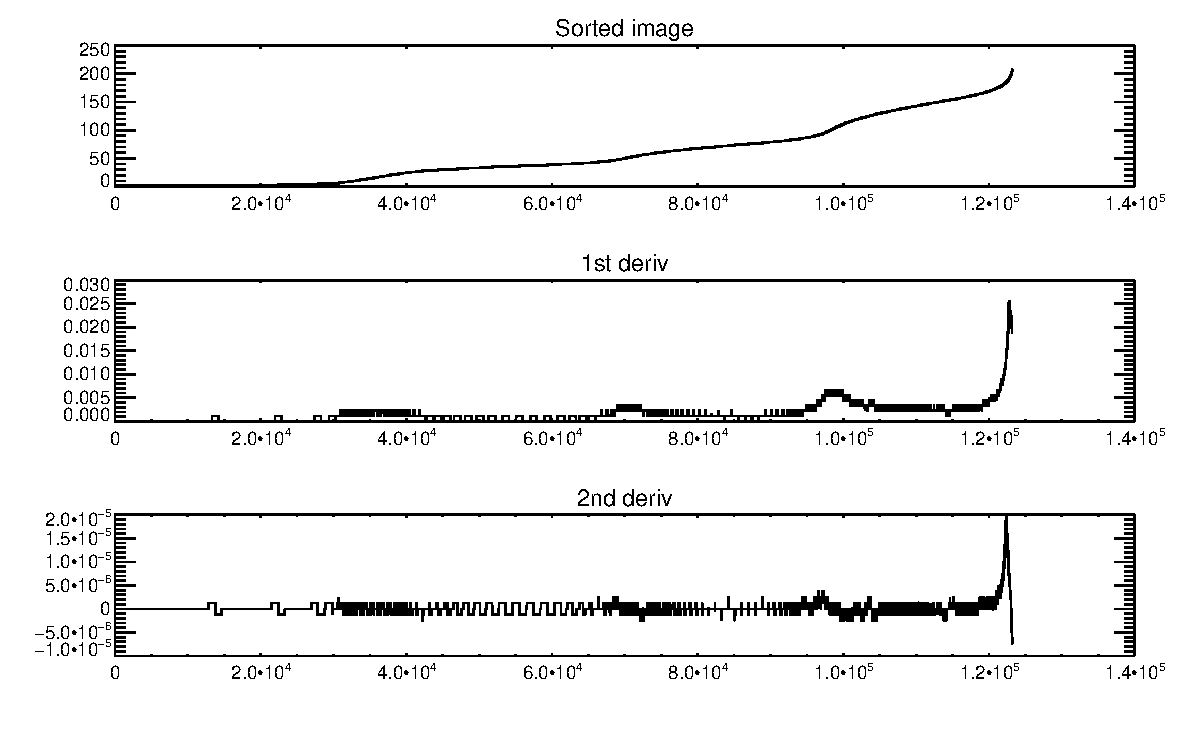
\includegraphics[width=.9\textwidth]{../plots_tables_images/sortedarray.eps}    
    \caption{We look at the second deriv because it consistently quantifies the thresholds to identify each solar region by. Unfortunately (or for better), we repeat this process per image we analyze. In terms of total time spent from starting the program to returning limb-fitted centers and fiducials, setting thresholds takes up about 25\%.}
    \label{sortedarray}
\end{figure}

\subsection{Possibility for Error} % (fold)
\label{sub:possibility_for_error}
Herein lies the problem of determining solar regions based on brightness and threshold values. We don't have a clear way of determining whether an image is dimmed before we even take a picture. If this happens, an image with a 100\% and 50\% sun may appear to be a 50\% and 25\% sun. There is no way to tell in our code, but hopefully we'll know enough about the time of day and pointing direction to account for this situation.
% subsection possibility_for_error (end)

% section setting_up_parameters (end)

\section{Prepare Image for Limb Fitting} % (fold)
\label{sec:prepare_image_for_limb_fitting}
After we set our threshold and parameters, we iteratively find and crop suns in the image. To determine if the sun is partially cut off, we create a border around the edge of our (usable) image. If the center is within the border, it is counted as a partial sun and excluded from further analysis. I emphasize \emph{usable} because the image's bottom two corners are cutoff, reducing the usable part of the image. Figure \ref{cuttingcorners} gives and example of what our mask might look like. The gradient is unimportant, it's purpose is only to emphasize the shape of the mask.

\begin{figure}[!ht]
    \ffigbox[][\FBheight]{%
    \begin{subfloatrow}[2]%
        \ffigbox[\FBwidth]%
       {%
       
\includegraphics[width=.5\textwidth]{../plots_tables_images/cutcorner.eps}%
       }%
       {%
       \caption{What our mask should look like - side of black triangle is 1/4 of image width}%
       \label{noborder}%
       }%
        \ffigbox[\Xhsize]%
       {%
       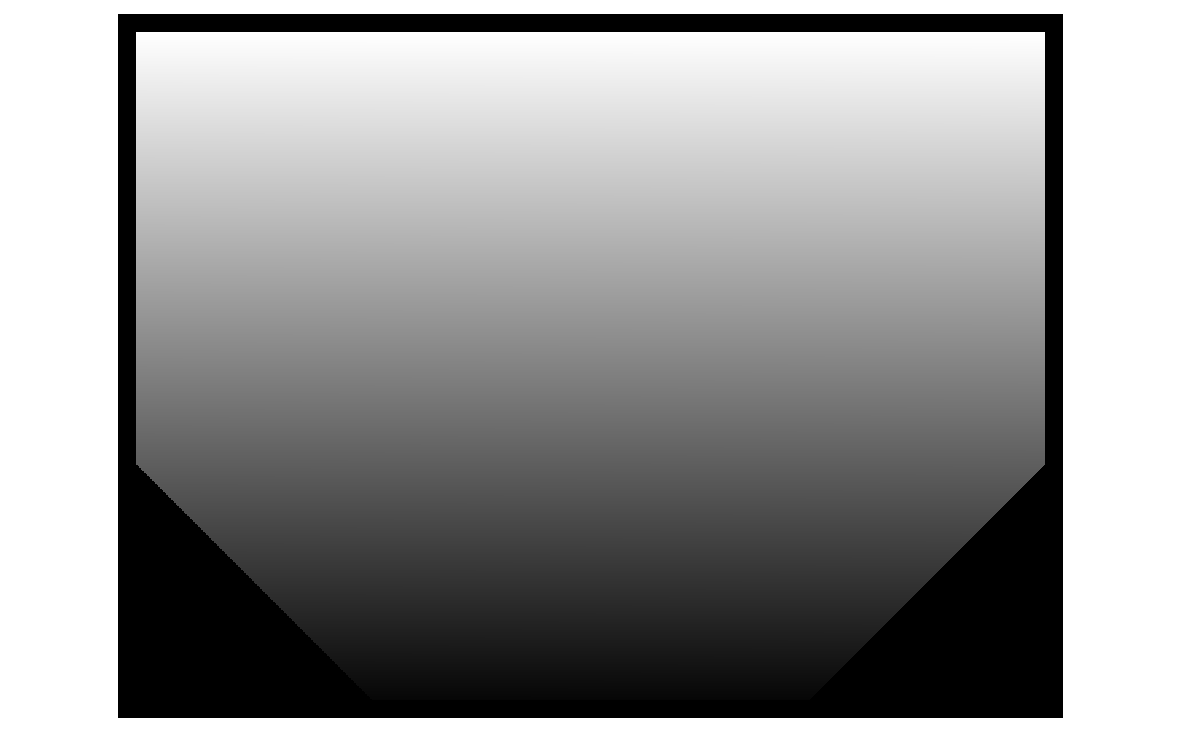
\includegraphics[width=.5\textwidth]{../plots_tables_images/cutcornerwborder.eps}%
       }%
       {%
       \caption{A proposed mask that looks within a certain distance form the border.}%
       \label{aborder}%
       }%
    \end{subfloatrow}}{\caption{The bottom corners will never see any data; the border mask takes into account the distance from the hypotenuse of the bottom corners}\label{cuttingcorners}}%
\end{figure}

% \begin{figure}[!ht]
%     \centering
%     \hspace{-1.0in}
%     \begin{subfigure}[b]{.45\linewidth}
%         \centering
%         
\includegraphics[width=1.3\textwidth]{../plots_tables_images/cutcorner.eps}
%         \caption{What our mask should look like - side of black triangle is 1/4 of image width}
%         \label{noborder}
%     \end{subfigure}
%     \hspace{.5in}
%     \begin{subfigure}[b]{.45\linewidth}
%         \centering
%         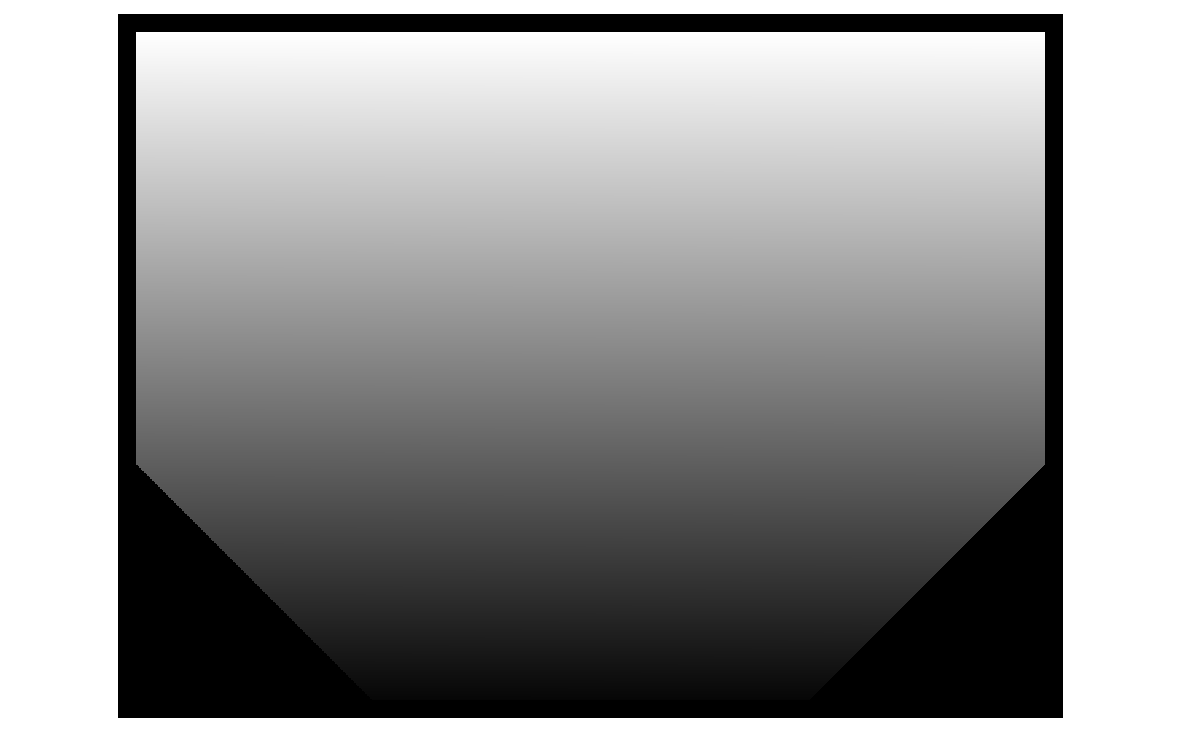
\includegraphics[width=1.3\textwidth]{../plots_tables_images/cutcornerwborder.eps}
%         \caption{A proposed mask that looks within a certain distance form the border.}
%         \label{aborder}
%     \end{subfigure}
%     \caption{The bottom corners will never see any data; the border mask takes into account the distance from the hypotenuse of the bottom corners}
%     \label{cuttingcorners}
% \end{figure}

% section prepare_image_for_limb_fitting (end)

\section{Fitting Limb Strips} % (fold)
\label{sec:fitting_limb_strips}

In order to fit limb strips, we first identify chords of the sun to take strips of. First, we look at the center of the sun and at regular intervals, choose rows/columns centered around the X/Y center position. The result are chords as seen in Figure \ref{chords}.\\
Now looking at each chord, we select 4 pixels around where the chord crosses a threshold; 2 pixels below the threshold and 2 pixels above. See Figure \ref{limbs}. One caveat is that if a fiducial is on the limb, our results may be skewed. This has been a persistent issue that we have not addressed fully yet.

\begin{figure}[!ht]
    \ffigbox[][\FBheight]{%
    \begin{subfloatrow}[2]%
        \ffigbox[\FBwidth]%
       {%
       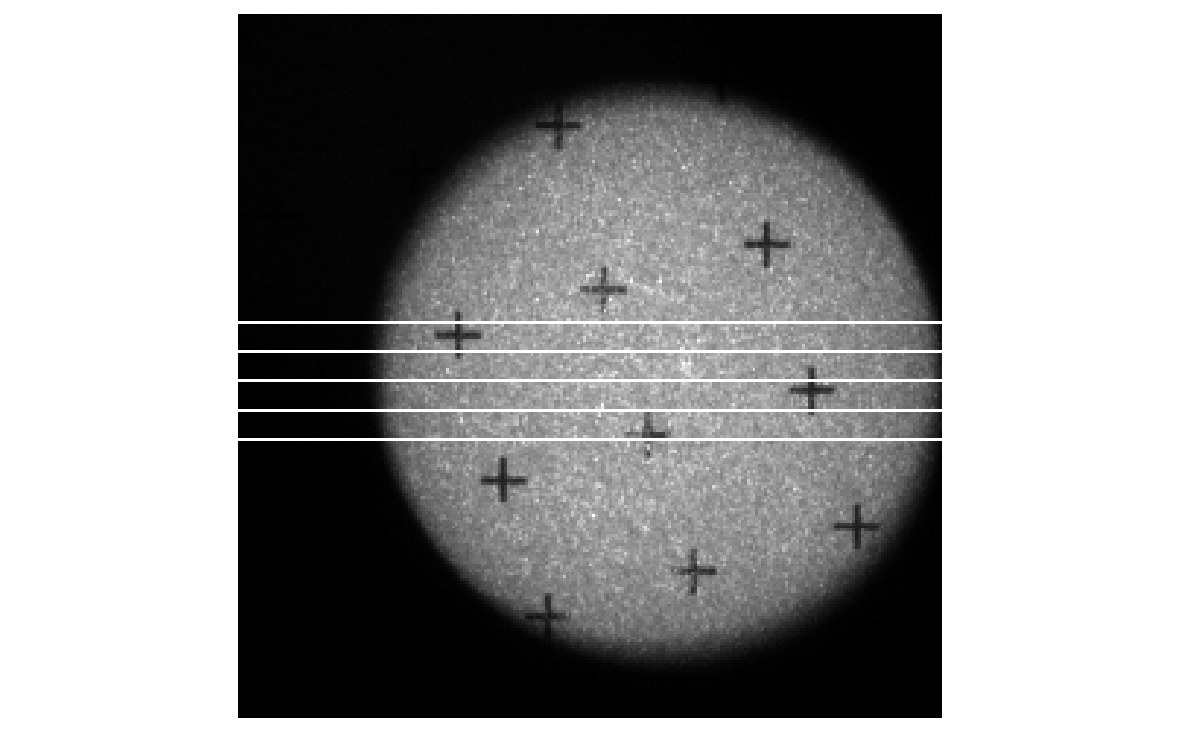
\includegraphics[width=.5\textwidth]{../plots_tables_images/5chords.eps}%
       }%
       {%
       \caption{The middle chord passes through the center of the sun}%
       \label{chords}%
       }%
        \ffigbox[\Xhsize]%
       {%
       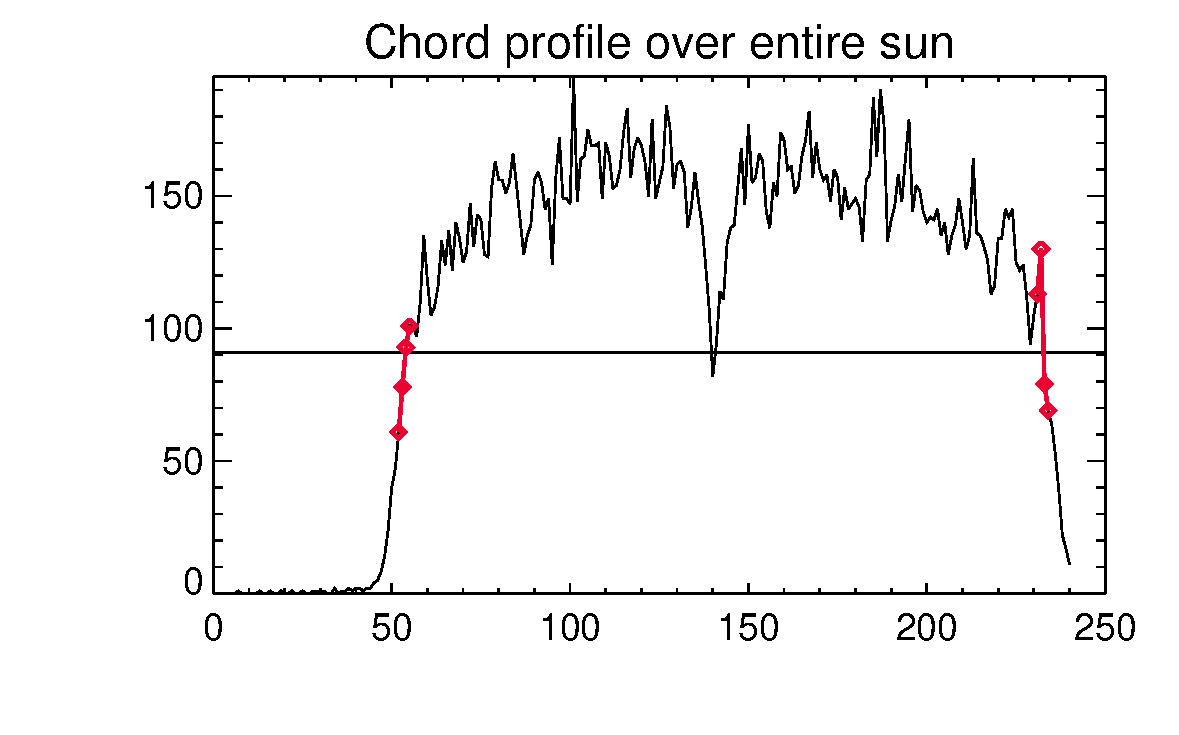
\includegraphics[width=.5\textwidth]{../plots_tables_images/redlimbs.eps}%
       }%
       {%
       \caption{The indices in red are the pixels we apply a linear fit to see where it crosses the threshold (which is the horizontal line).}%
       \label{limbs}%
       }%
    \end{subfloatrow}}{\caption{}\label{sup}}%
\end{figure}

% \begin{figure}[!ht]
%     \centering
%     \hspace{-1.0in}
%     \begin{subfigure}[b]{.45\linewidth}
%         \centering
%         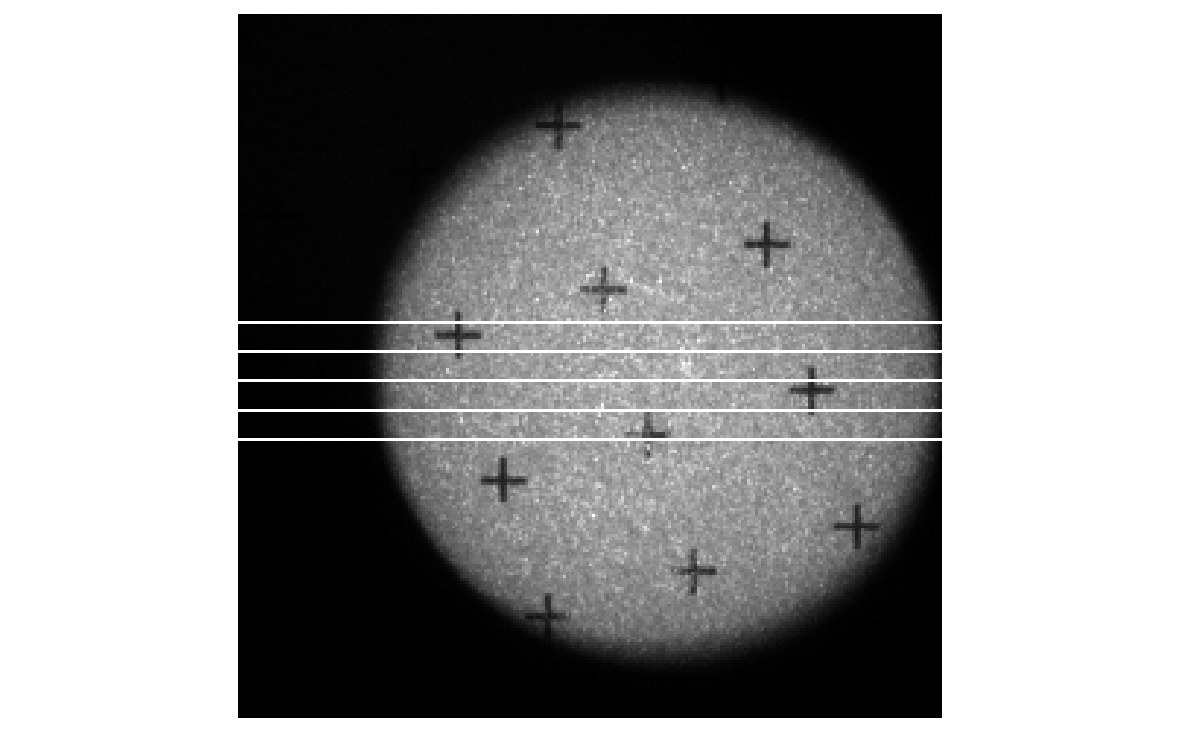
\includegraphics[width=.9\textwidth]{../plots_tables_images/5chords.eps}
%         \caption{The middle chord passes through the center of the sun}
%         \label{chords}
%     \end{subfigure}
%     \hspace{.5in}
%     \begin{subfigure}[b]{.45\linewidth}
%         \centering
%         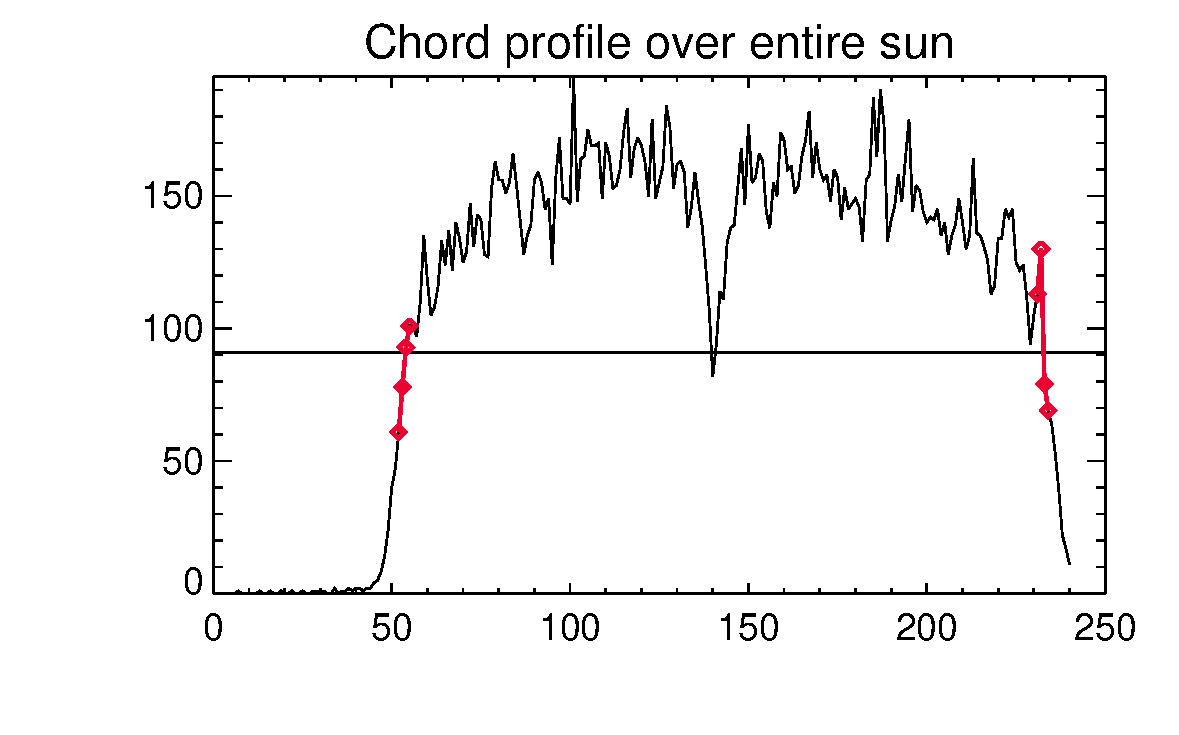
\includegraphics[width=1.3\textwidth]{../plots_tables_images/redlimbs.eps}
%         \caption{The indices in red are the pixels we apply a linear fit to see where it crosses the threshold (which is the horizontal line).}
%         \label{limbs}
%     \end{subfigure}
%     \caption{}
%     \label{sup}
% \end{figure}

% section fitting_limb_strips (end)

\section{Finding Fiducials} % (fold)
\label{sec:finding_fiducials}

\begin{figure}[!ht]
    \ffigbox[][\FBheight]{%
    \begin{subfloatrow}[2]%
        \ffigbox[\FBwidth]%
       {%
       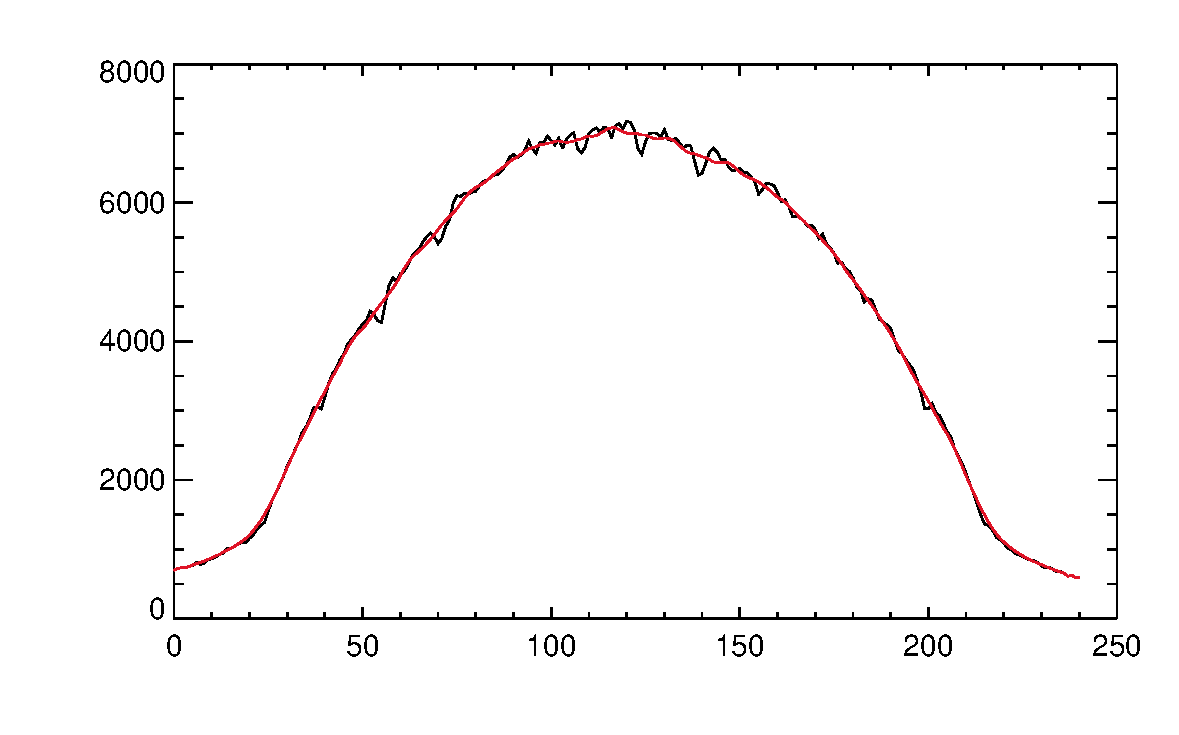
\includegraphics[width=.5\textwidth]{../plots_tables_images/smooth_expl.eps}%
       }%
       {%
       \caption{This is the 1D sum of a solar image. Small dips are seen in the profile corresponding to fiducials. The line in red is the sum smoothed by 10 pixels.}%
       \label{doublelines}%
       }%
        \ffigbox[\Xhsize]%
       {%
       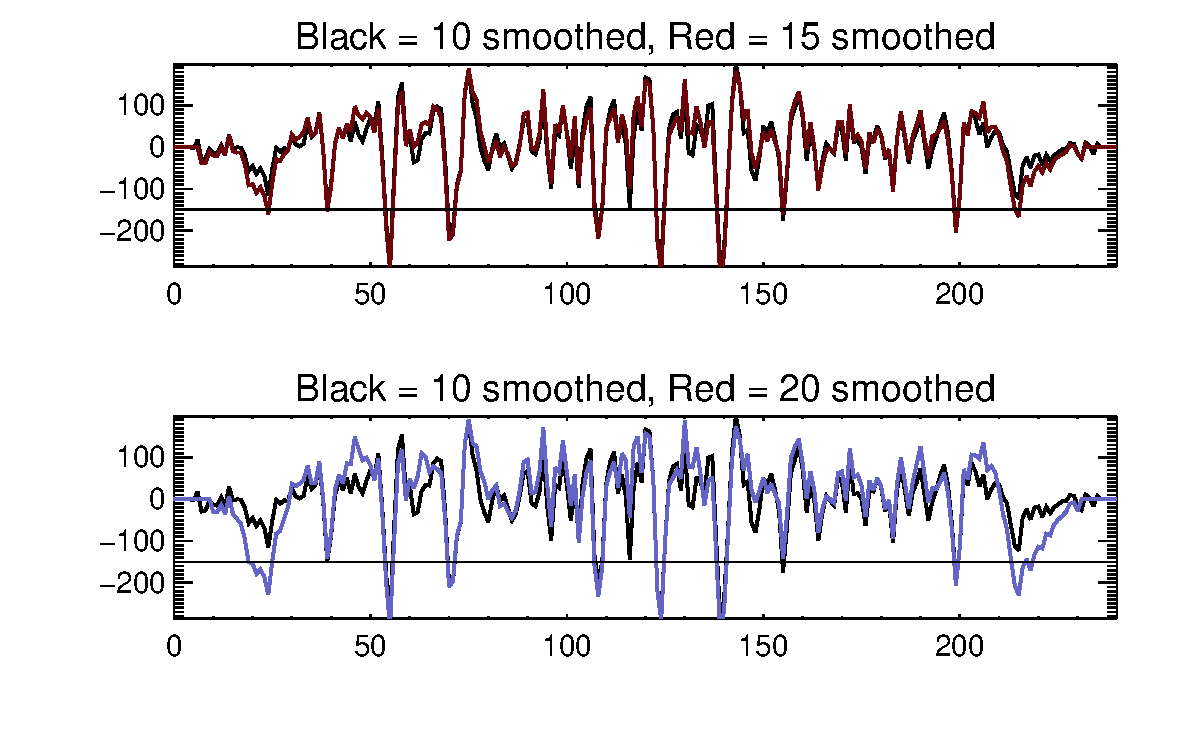
\includegraphics[width=.5\textwidth]{../plots_tables_images/smoothcomp.eps}%
       }%
       {%
       \caption{We subtract the smoothed profile from the raw data to emphasize dips. Comparisons of the smooth amount change the width and number of the dips, although not really the depth.}%
       \label{threshed}%
       }%
    \end{subfloatrow}}{\caption{}\label{smoothed}}%
\end{figure}

% \begin{figure}[!ht]
%     \begin{subfigure}[b]{.5\linewidth}
%         \centering
%         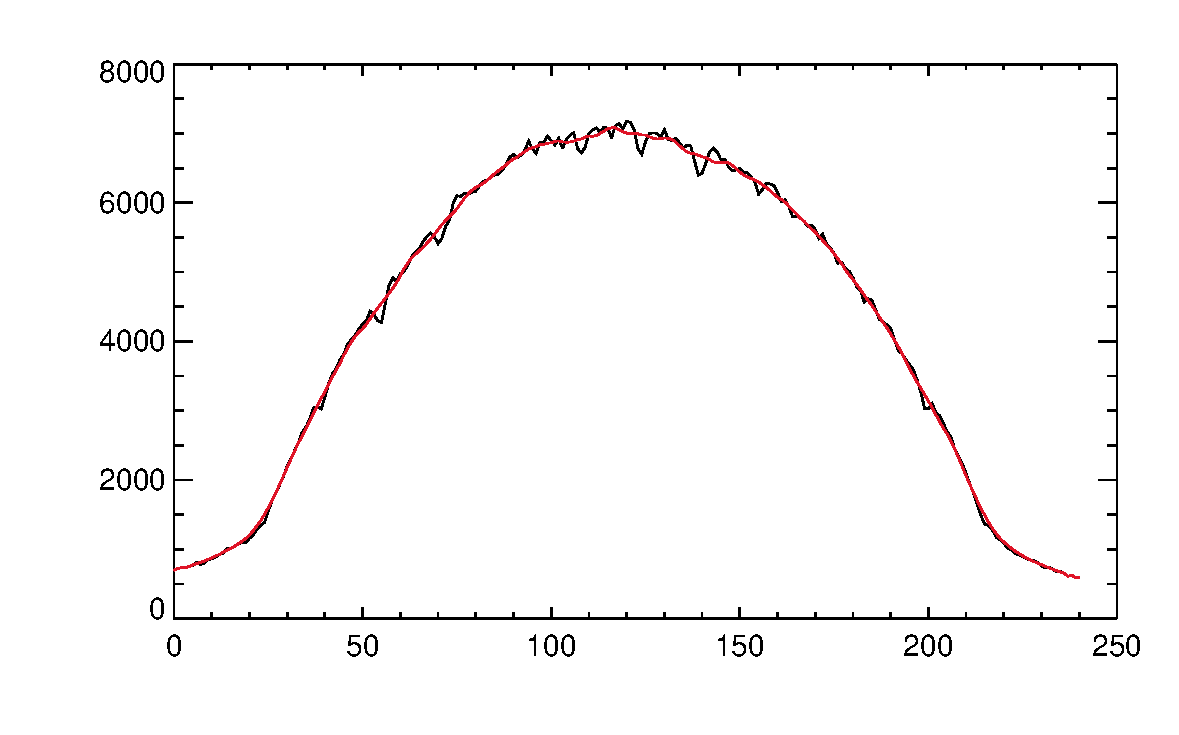
\includegraphics[width=\linewidth]{../plots_tables_images/smooth_expl.eps}
%         \caption{This is the 1D sum of a solar image. Small dips are seen in the profile corresponding to fiducials. The line in red is the sum smoothed by 10 pixels.}
%         \label{doublelines}
%     \end{subfigure}
%     \begin{subfigure}[b]{.5\linewidth}
%         \centering
%         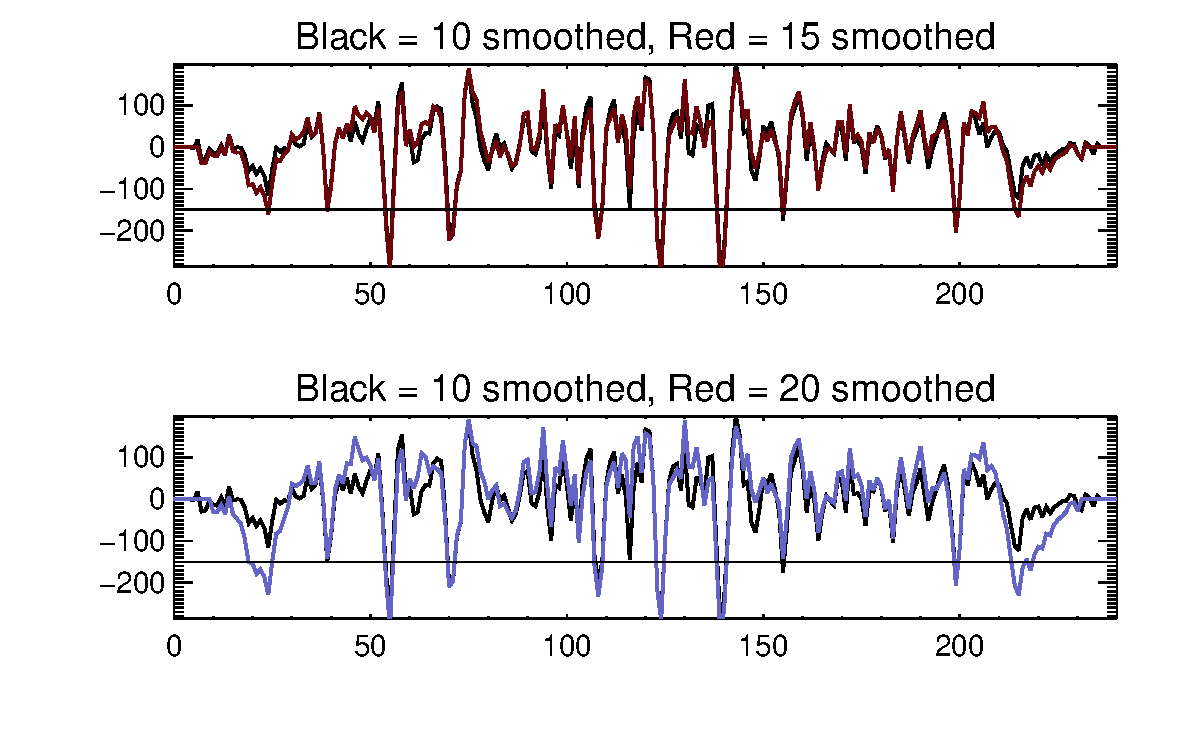
\includegraphics[width=\linewidth]{../plots_tables_images/smoothcomp.eps}
%         \caption{We subtract the smoothed profile from the raw data to emphasize dips. Comparisons of the smooth amount change the width and number of the dips, although not really the depth.}
%         \label{threshed}
%     \end{subfigure}
%     \caption{}
%     \label{smoothed}
% \end{figure}

Once we have a limb-fitted center, we crop a box around the center so that the sun sits comfortable inside without being clipped at the edges. We then find the sum of the image in 1D; i.e., summing the rows/columns. Certain rows/columns will have a dip in their sum (see black line in Figure \ref{doublelines}) from a fiducial. We smooth the sum (see red line in Figure \ref{doublelines}) and then subtract the two so that we have peaks at rows/columns of fiducials. (See Figure \ref{threshed}) Since we don't know which pairs of coordinates go with each other, we look at all possibilities. \\

For each position below a certain threshold (see Figure \ref{threshed}) a row/column  is returned. Once we have an array of possible fiducial row and column positions, we look at each pair of coordinates to check if it is a fiducial. Our first check is to make sure the pixel value at the fiducial candidate is sufficiently dim. Many pairs end up on the solar disk but not on a fiducial. Then, we look at the 1D sum of a cropped region around a fiducial candidate. If there is a clear, whole fiducial in the cropped region, there should be dips in the 1D sum. We smooth the 1D sum and subtract it from itself to find peaks. If these peaks are above a certain threshold (100 in Figure \ref{lotsofplot}) in each axis, then the fiducial candidate is considered a \emph{real} fiducial. Figure \ref{lotsofcrop} illustrates what each fiducial candidate looks like for a certain sun. 

\begin{figure}[!ht]
\vspace{-0.5in}
    \ffigbox[][\FBheight]{%
    \begin{subfloatrow}[3]%
        \ffigbox[\FBwidth]%
        {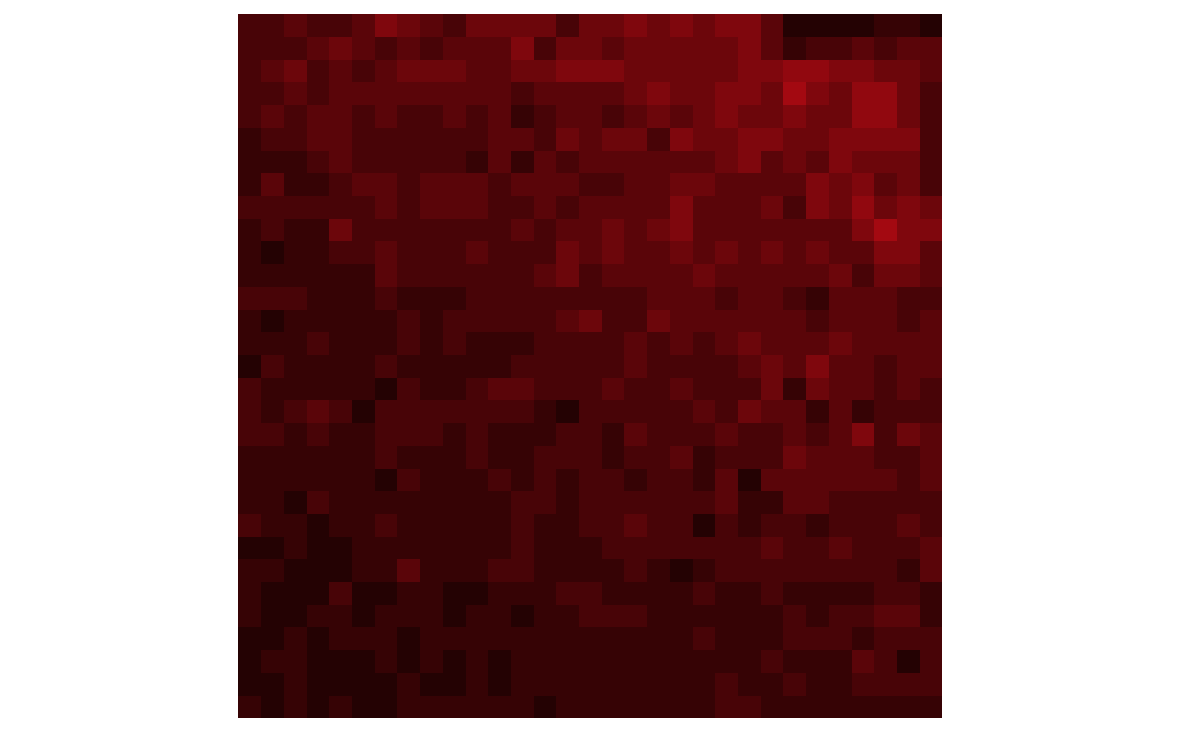
\includegraphics[width=.3\textwidth]{../plots_tables_images/1d1dcrop_0_0.eps}}{}%
        \ffigbox[\FBwidth]%
        {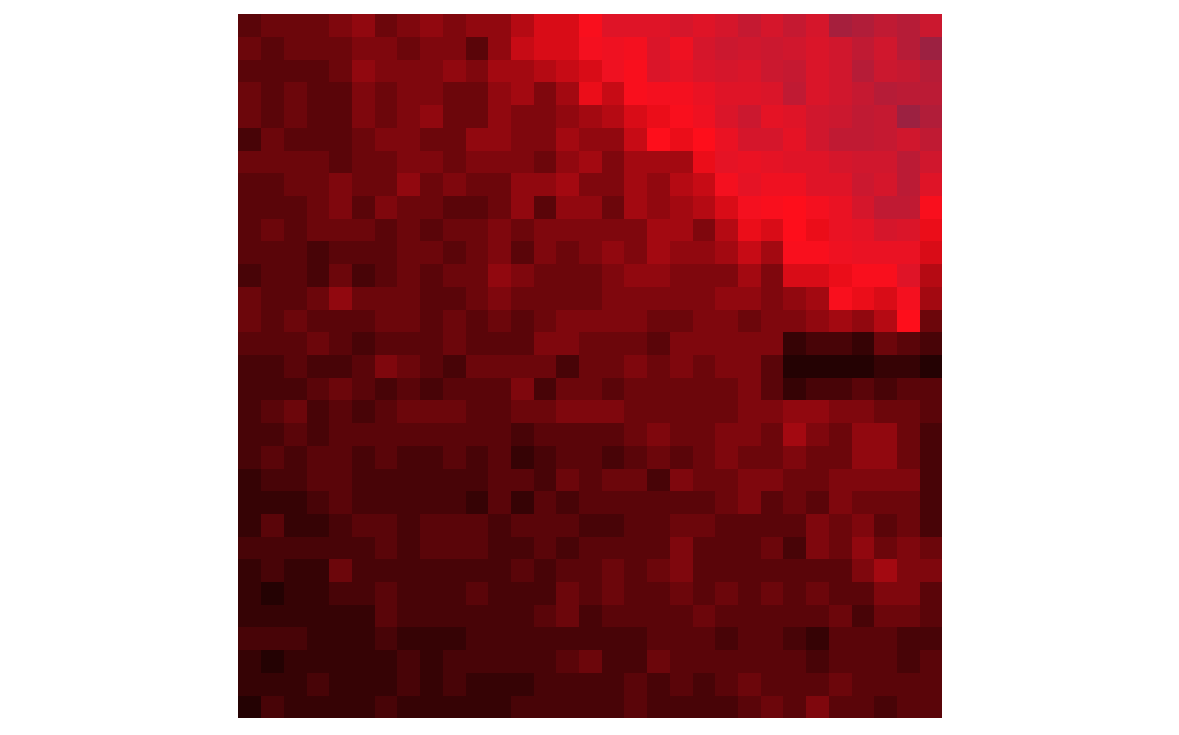
\includegraphics[width=.3\textwidth]{../plots_tables_images/1d1dcrop_0_1.eps}}{}%
        \ffigbox[\FBwidth]%
        {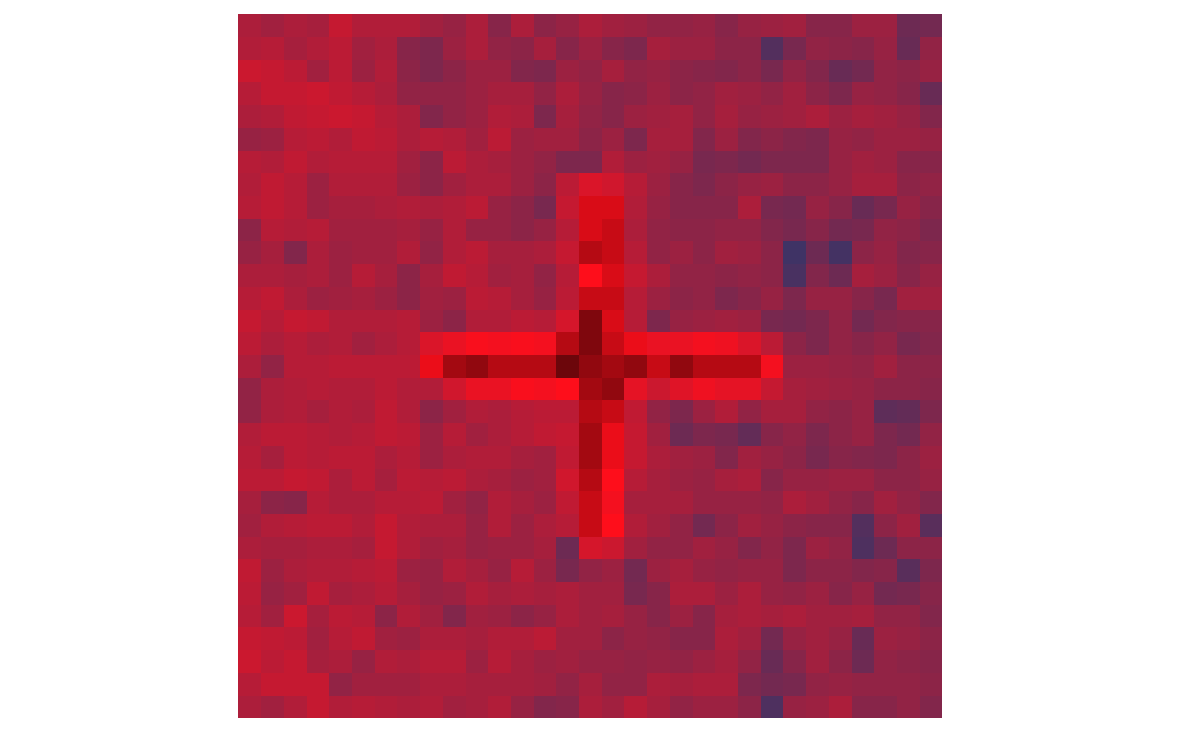
\includegraphics[width=.3\textwidth]{../plots_tables_images/1d1dcrop_0_4.eps}}{}%
    \end{subfloatrow}}

    \ffigbox[][\FBheight]{%
    \begin{subfloatrow}[3]%
        \ffigbox[\FBwidth]%
        {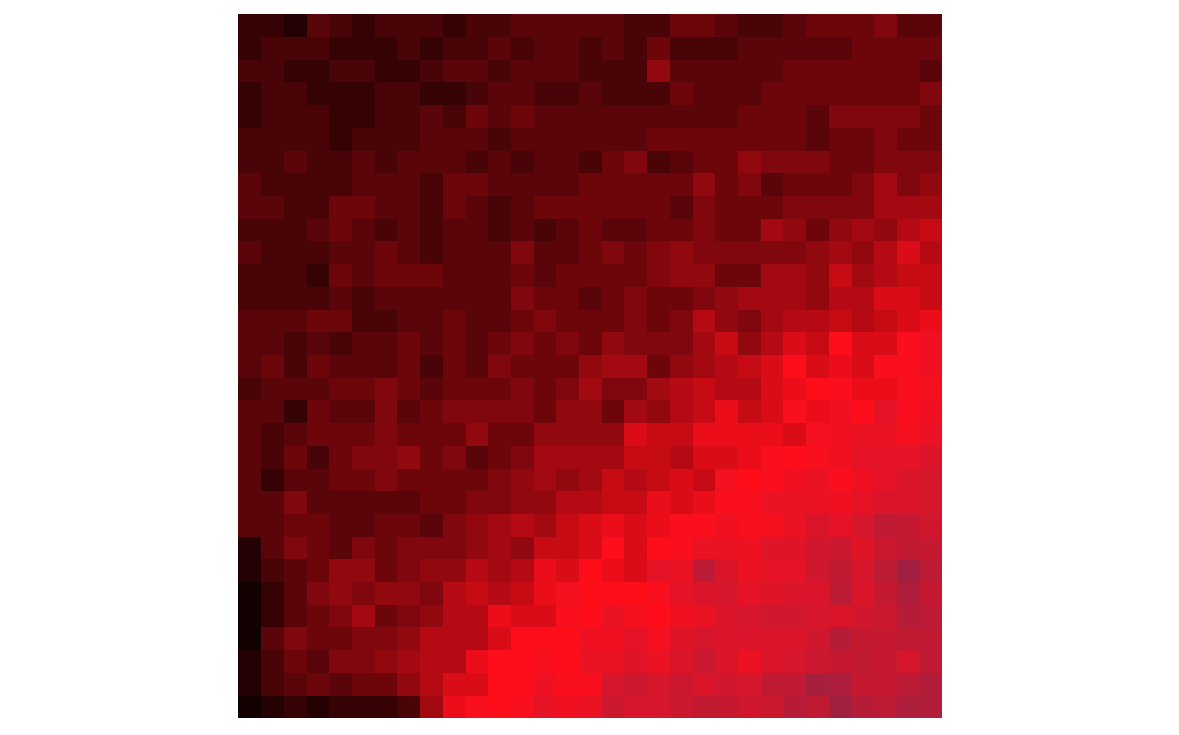
\includegraphics[width=.3\textwidth]{../plots_tables_images/1d1dcrop_0_8.eps}}{}%
        \ffigbox[\FBwidth]%
        {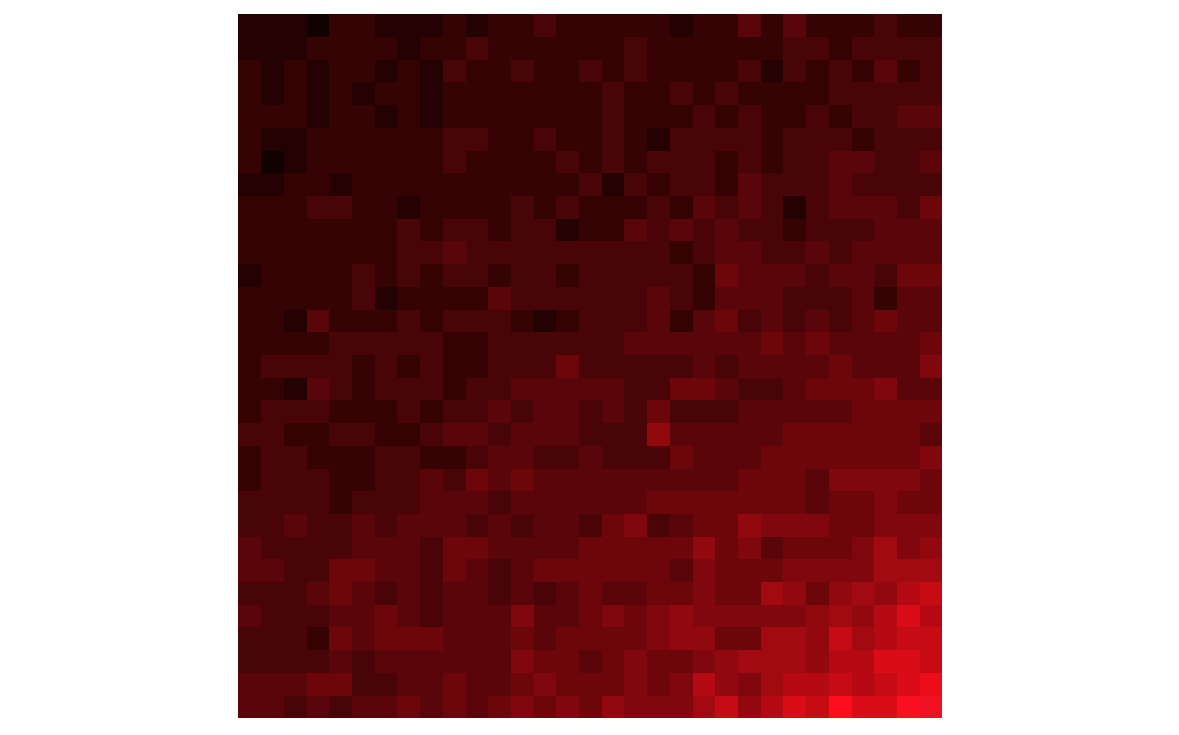
\includegraphics[width=.3\textwidth]{../plots_tables_images/1d1dcrop_0_9.eps}}{}%
        \ffigbox[\FBwidth]%
        {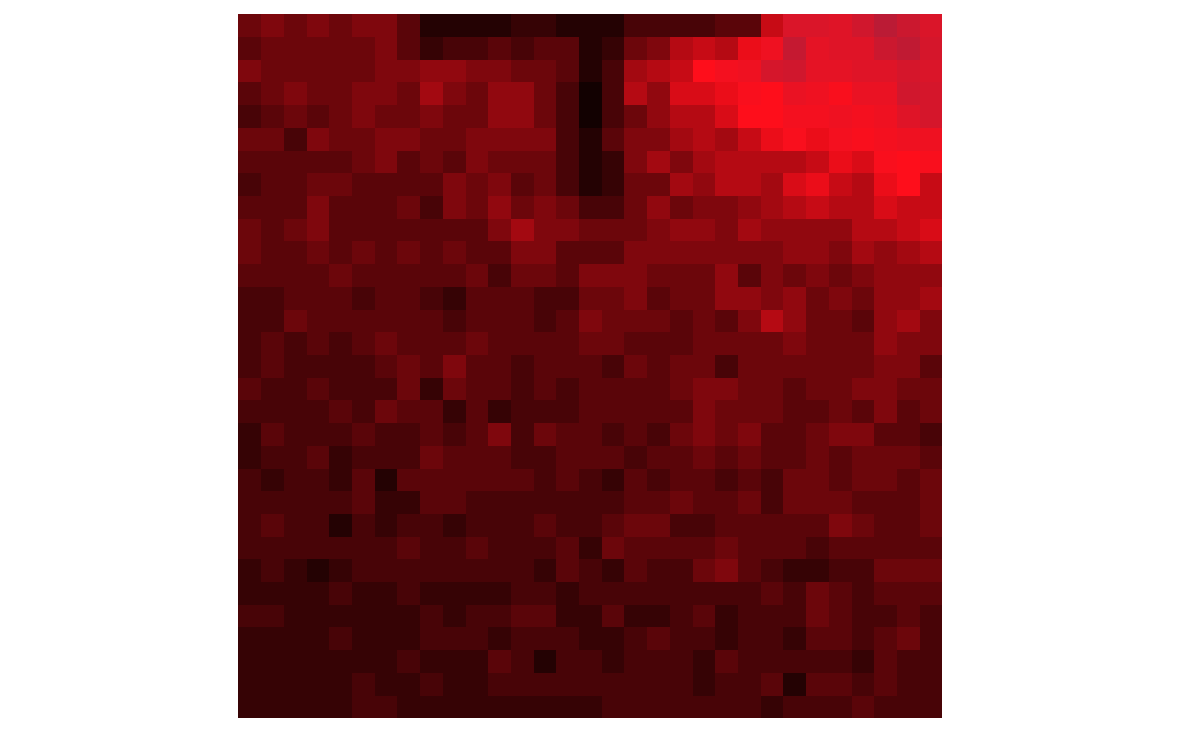
\includegraphics[width=.3\textwidth]{../plots_tables_images/1d1dcrop_1_0.eps}}{}%
    \end{subfloatrow}}

    \ffigbox[][\FBheight]{%
    \begin{subfloatrow}[3]%
        \ffigbox[\FBwidth]%
        {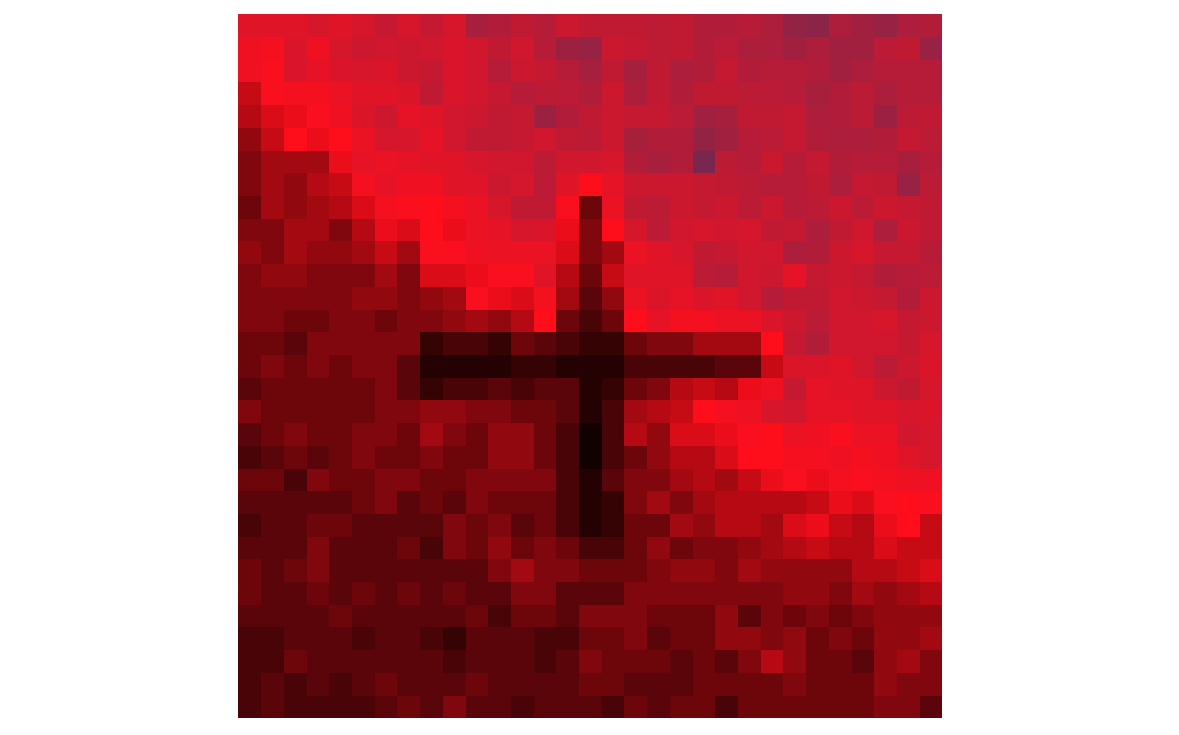
\includegraphics[width=.3\textwidth]{../plots_tables_images/1d1dcrop_1_1.eps}}{}%
        \ffigbox[\FBwidth]%
        {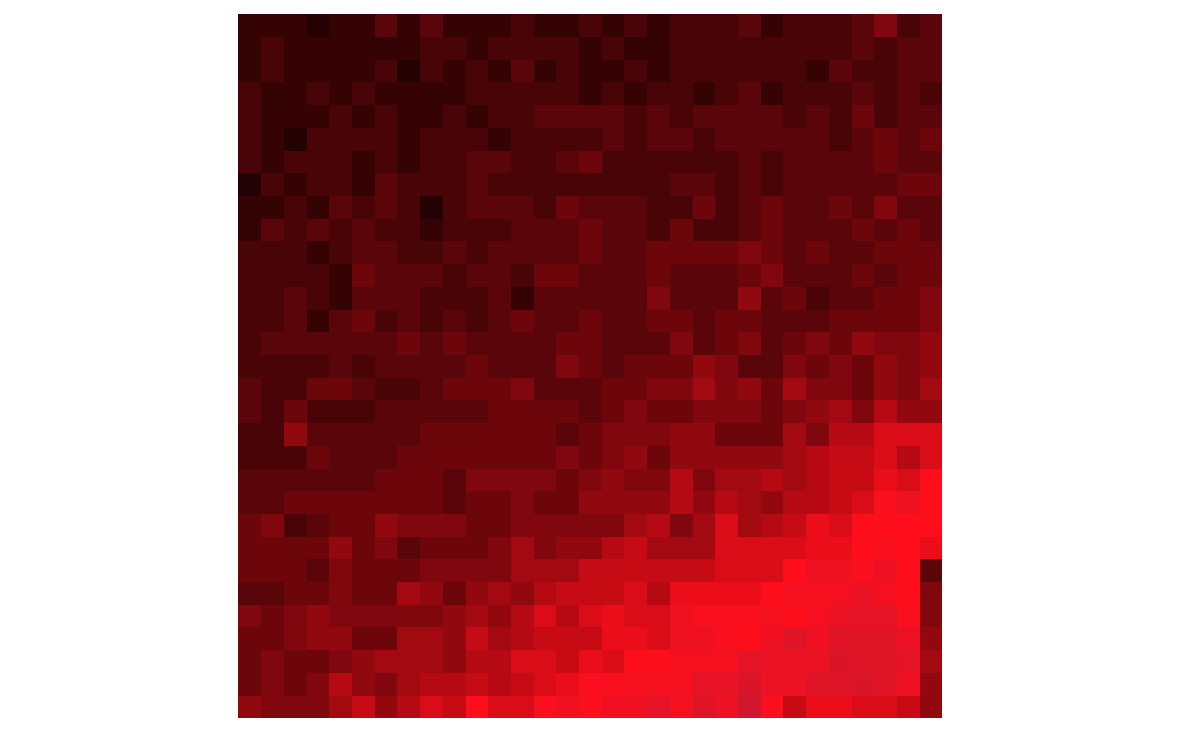
\includegraphics[width=.3\textwidth]{../plots_tables_images/1d1dcrop_1_9.eps}}{}%
        \ffigbox[\FBwidth]%
        {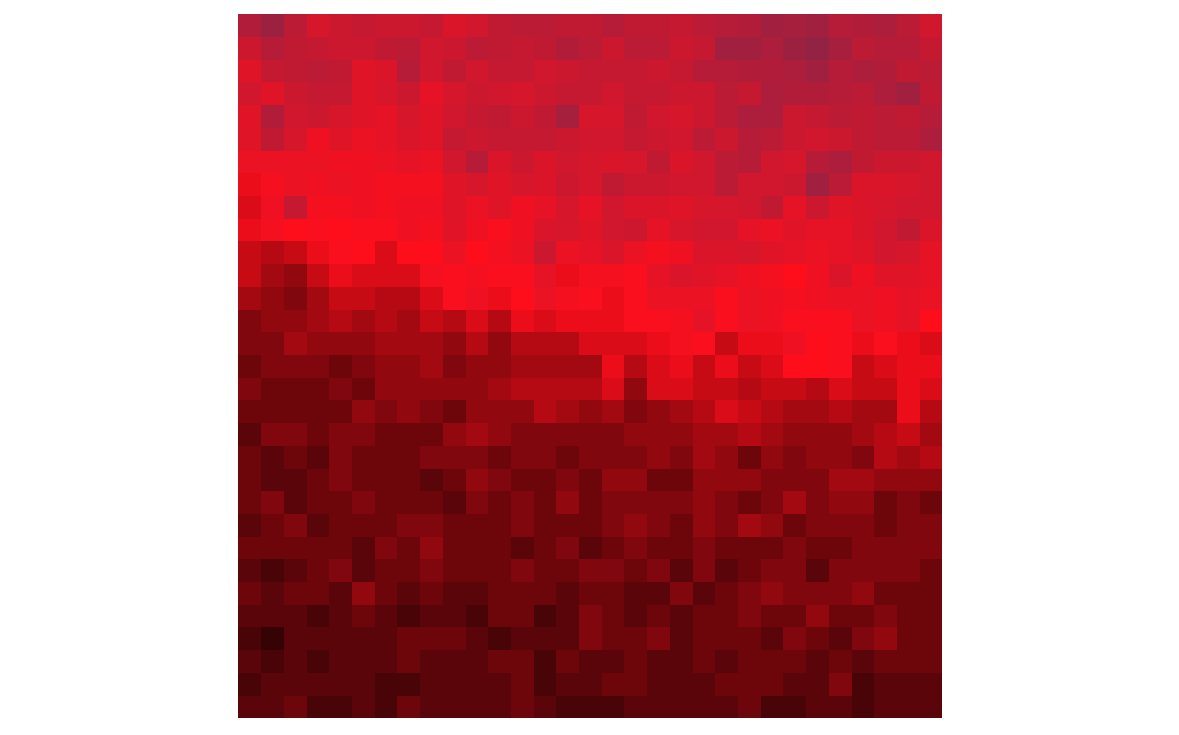
\includegraphics[width=.3\textwidth]{../plots_tables_images/1d1dcrop_2_0.eps}}{}%
    \end{subfloatrow}}

    \ffigbox[][\FBheight]{%
    \begin{subfloatrow}[3]%
        \ffigbox[\FBwidth]%
        {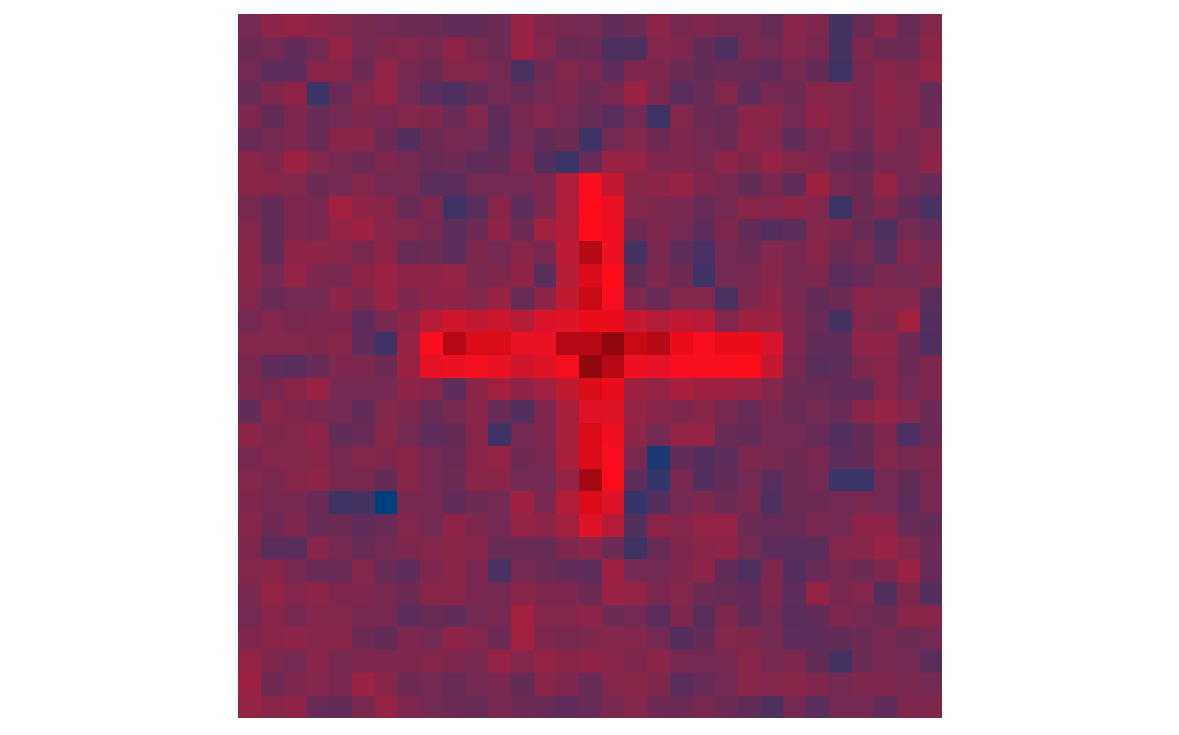
\includegraphics[width=.3\textwidth]{../plots_tables_images/1d1dcrop_2_5.eps}}{}%
        \ffigbox[\FBwidth]%
        {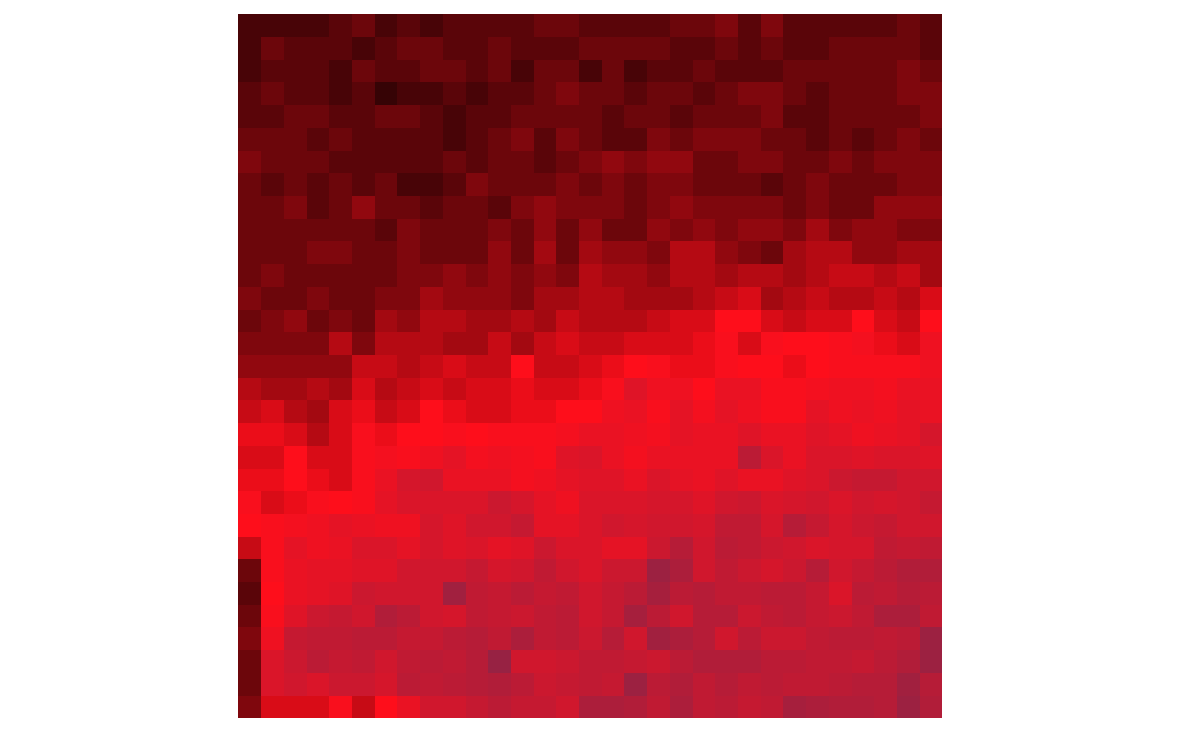
\includegraphics[width=.3\textwidth]{../plots_tables_images/1d1dcrop_2_9.eps}}{}%
        \ffigbox[\FBwidth]%
        {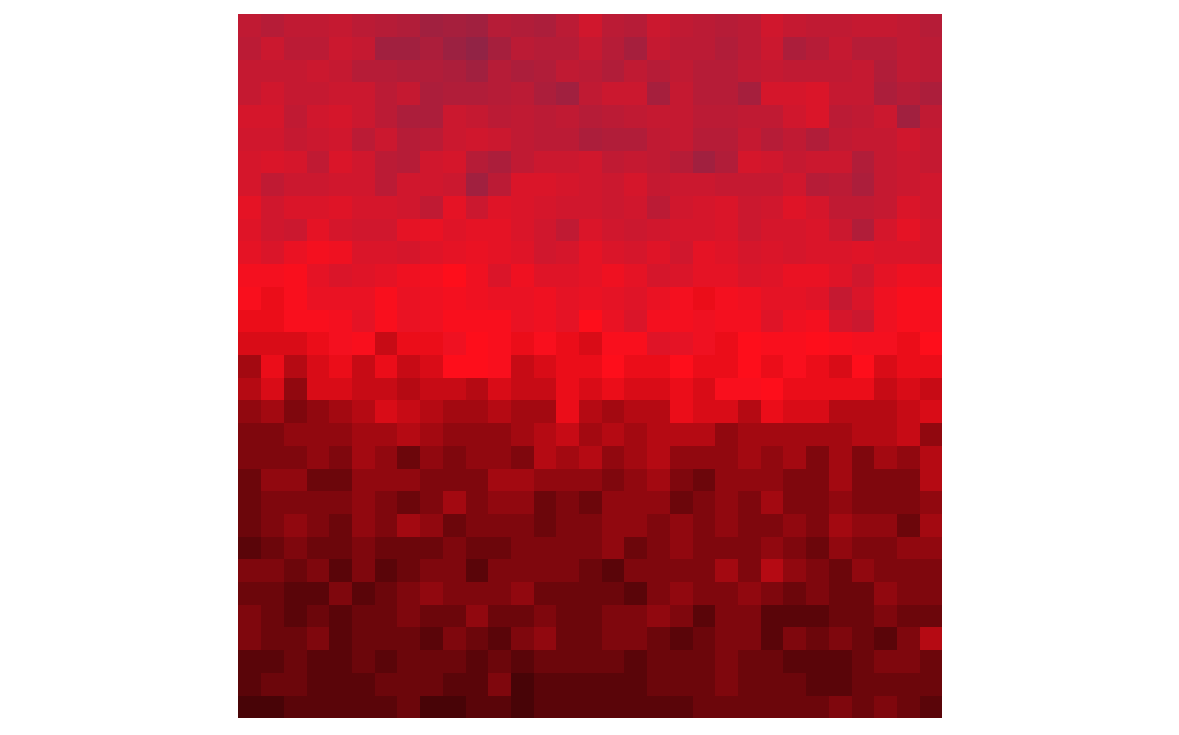
\includegraphics[width=.3\textwidth]{../plots_tables_images/1d1dcrop_3_0.eps}}{}%
    \end{subfloatrow}}

    \ffigbox[][\FBheight]{%
    \begin{subfloatrow}[3]%
        \ffigbox[\FBwidth]%
        {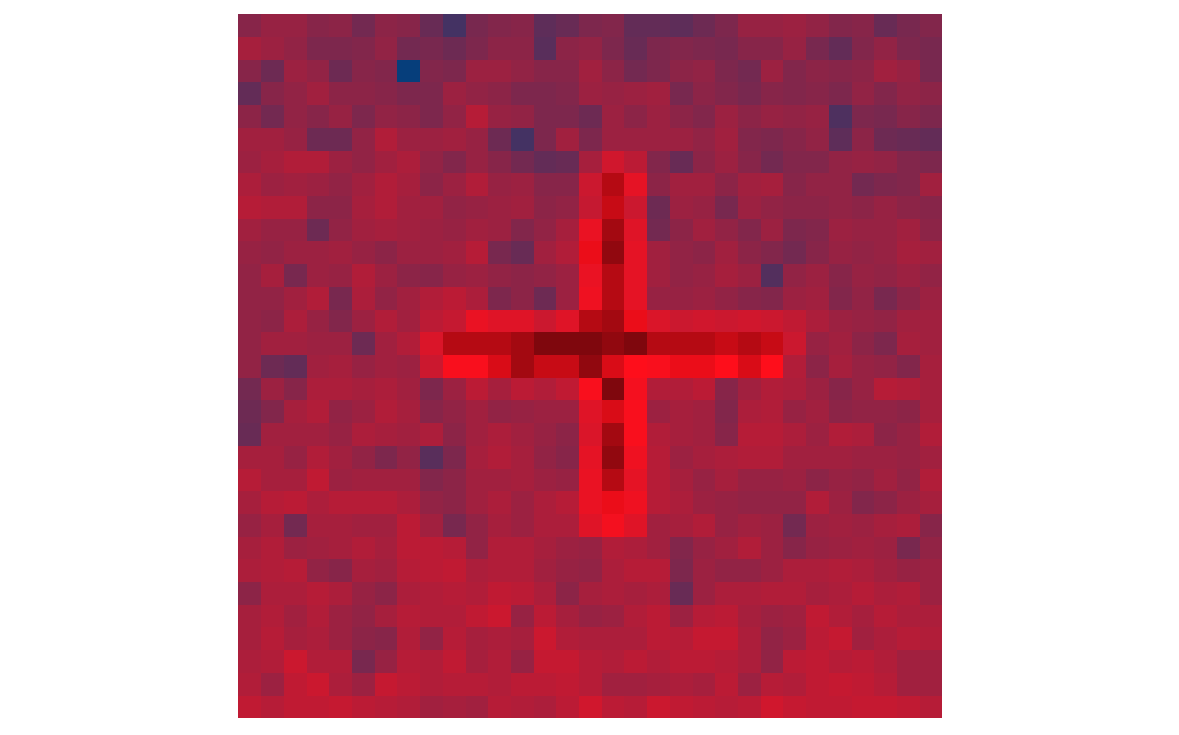
\includegraphics[width=.3\textwidth]{../plots_tables_images/1d1dcrop_3_2.eps}}{}%
        \ffigbox[\FBwidth]%
        {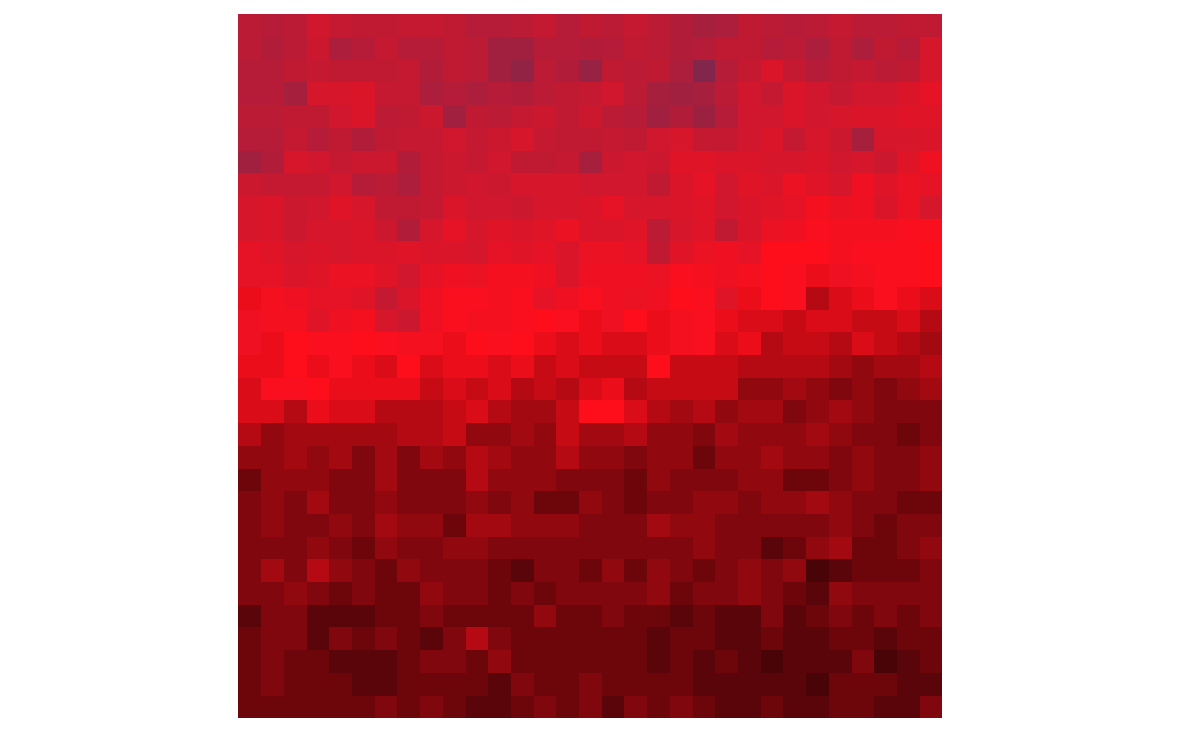
\includegraphics[width=.3\textwidth]{../plots_tables_images/1d1dcrop_4_0.eps}}{}%
        \ffigbox[\FBwidth]%
        {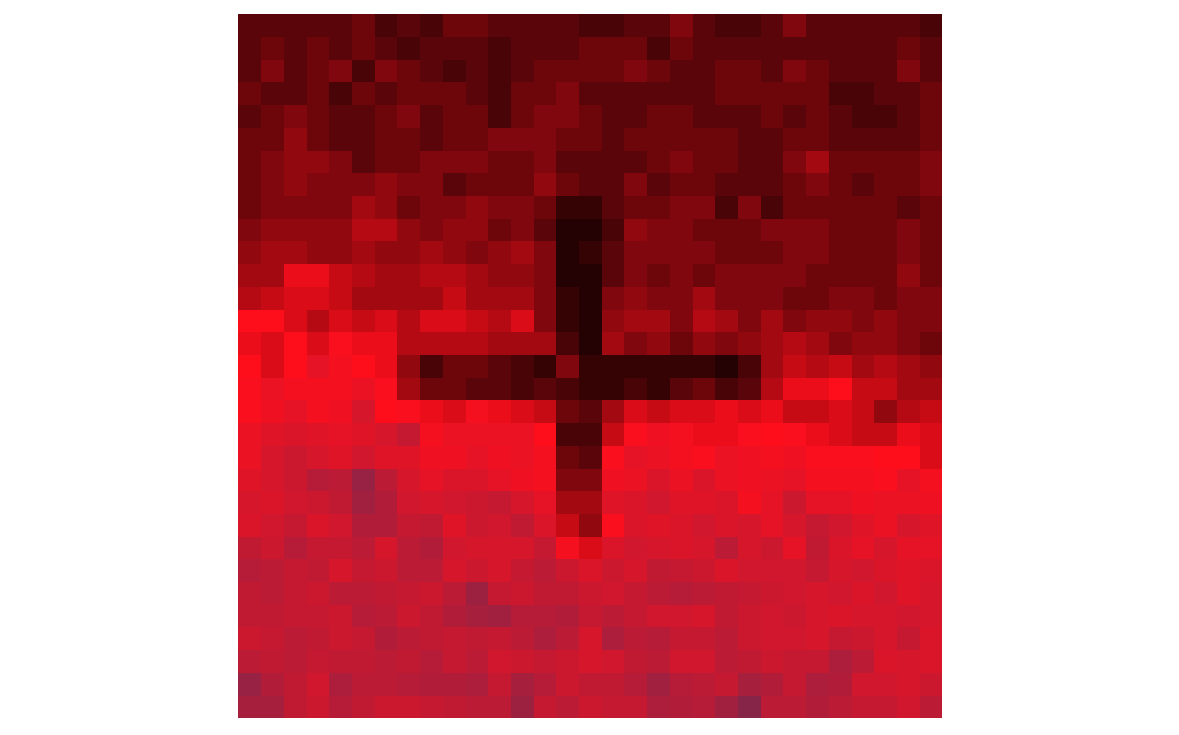
\includegraphics[width=.3\textwidth]{../plots_tables_images/1d1dcrop_4_9.eps}}{}%
    \end{subfloatrow}}

    \ffigbox[][\FBheight]{%
    \begin{subfloatrow}[3]%
        \ffigbox[\FBwidth]%
        {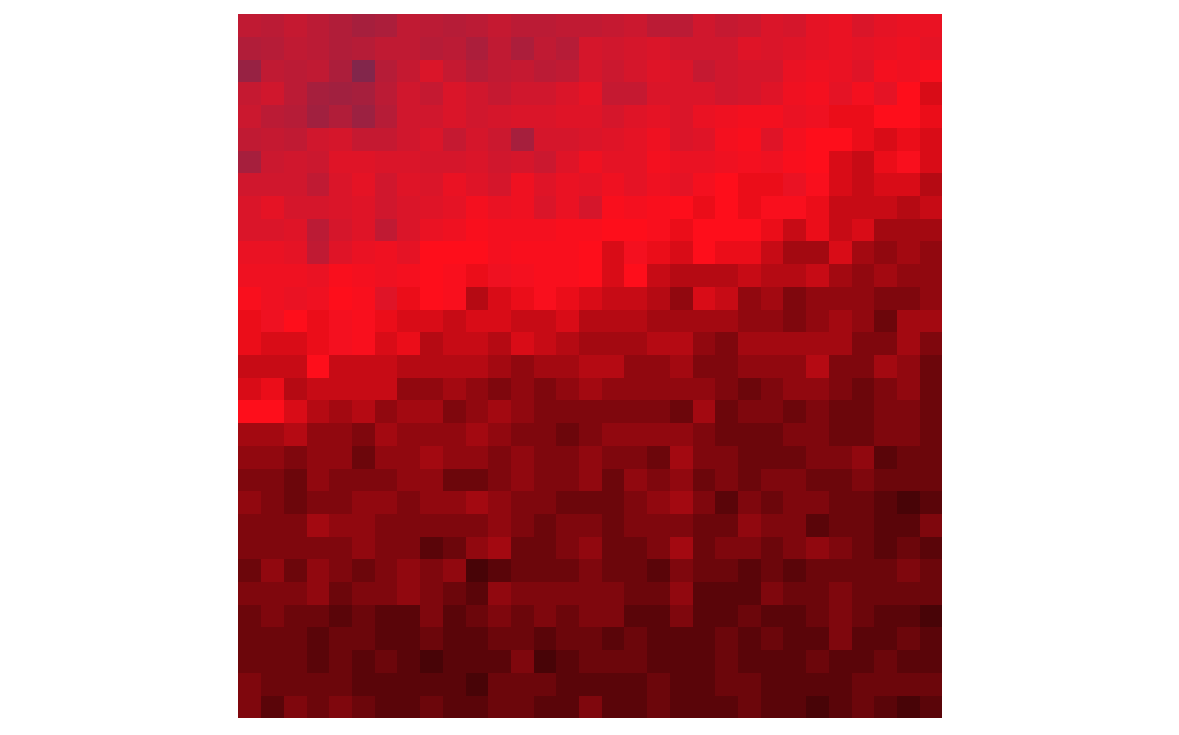
\includegraphics[width=.3\textwidth]{../plots_tables_images/1d1dcrop_5_0.eps}}{}%
        \ffigbox[\FBwidth]%
        {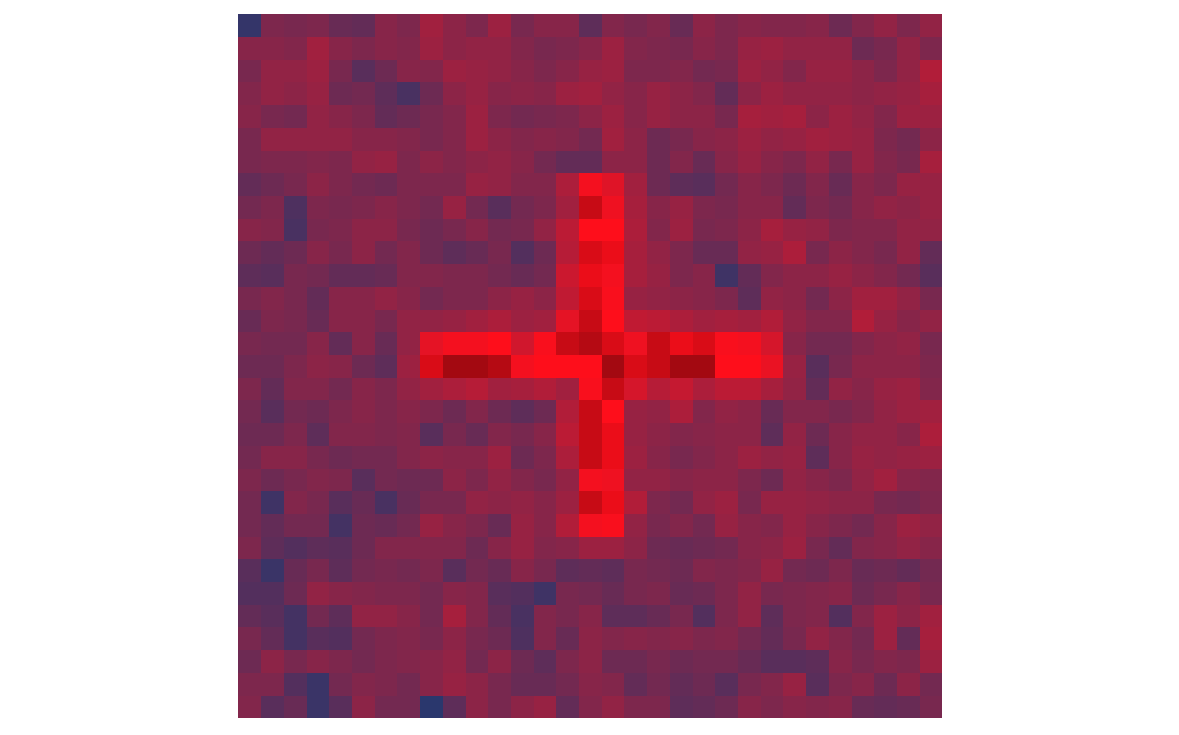
\includegraphics[width=.3\textwidth]{../plots_tables_images/1d1dcrop_5_6.eps}}{}%
        \ffigbox[\FBwidth]%
        {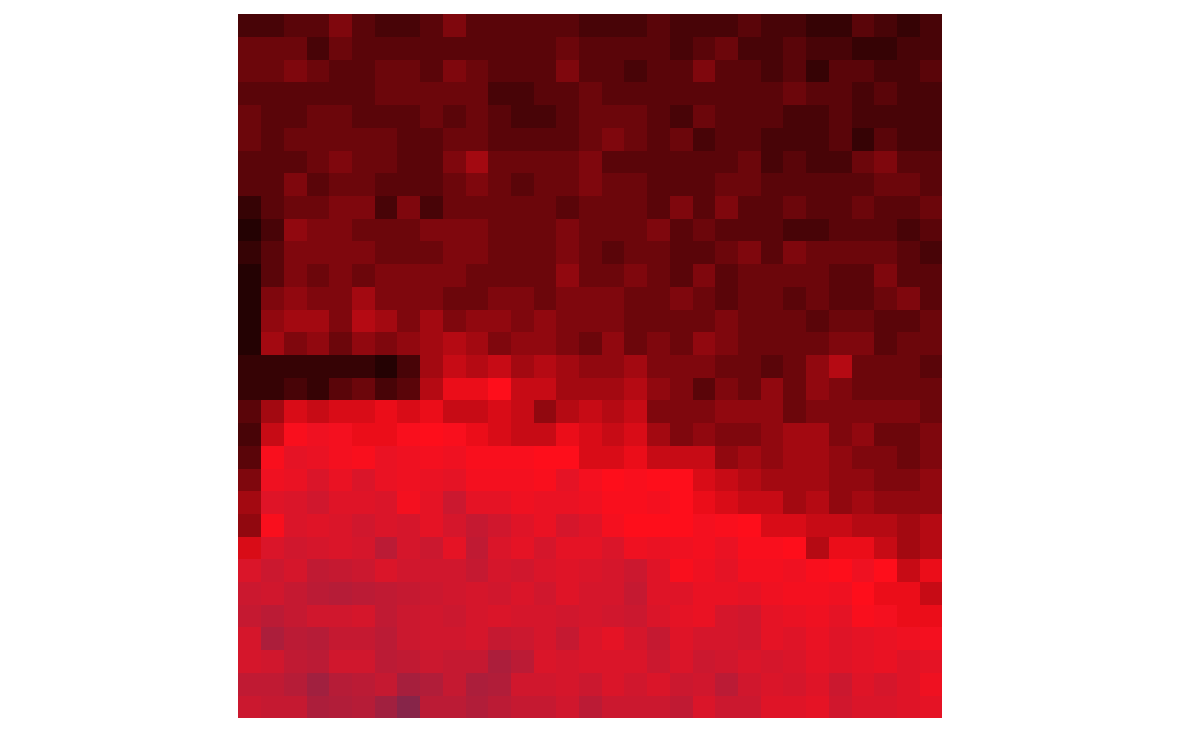
\includegraphics[width=.3\textwidth]{../plots_tables_images/1d1dcrop_5_9.eps}}{}%
    \end{subfloatrow}}

    \ffigbox[][\FBheight]{%
    \begin{subfloatrow}[3]%
        \ffigbox[\FBwidth]%
        {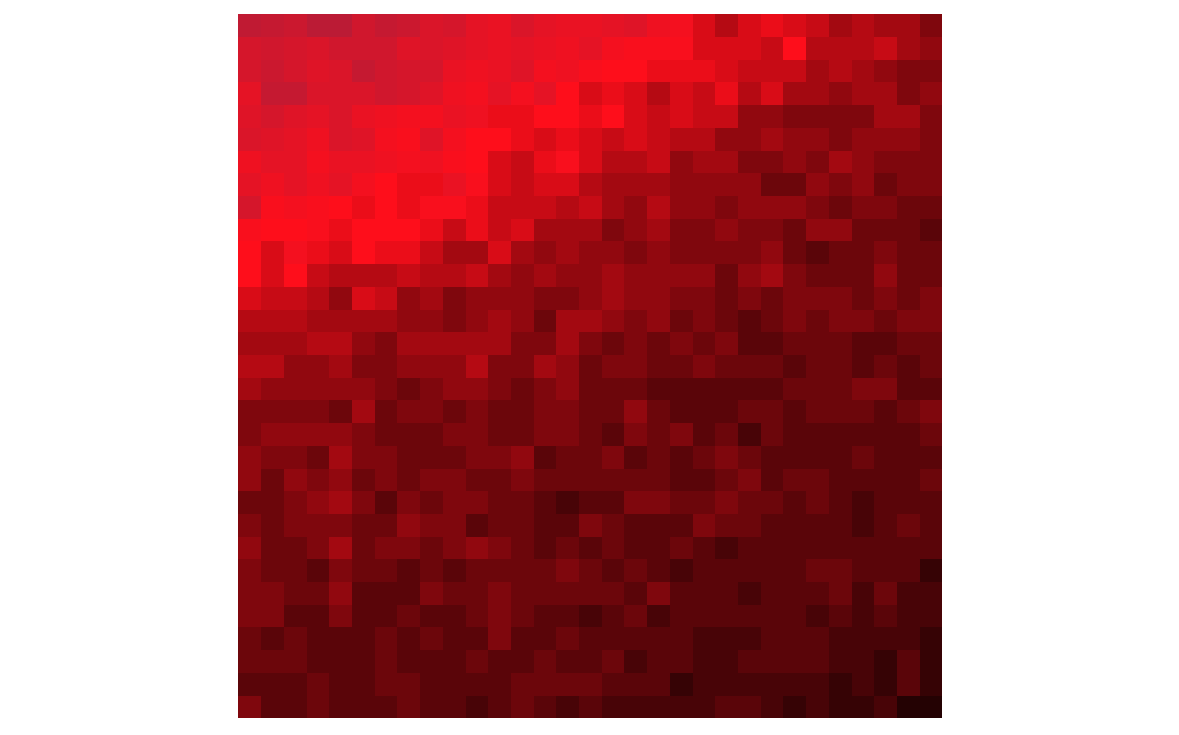
\includegraphics[width=.3\textwidth]{../plots_tables_images/1d1dcrop_6_0.eps}}{\caption{}}%
        \ffigbox[\FBwidth]%
        {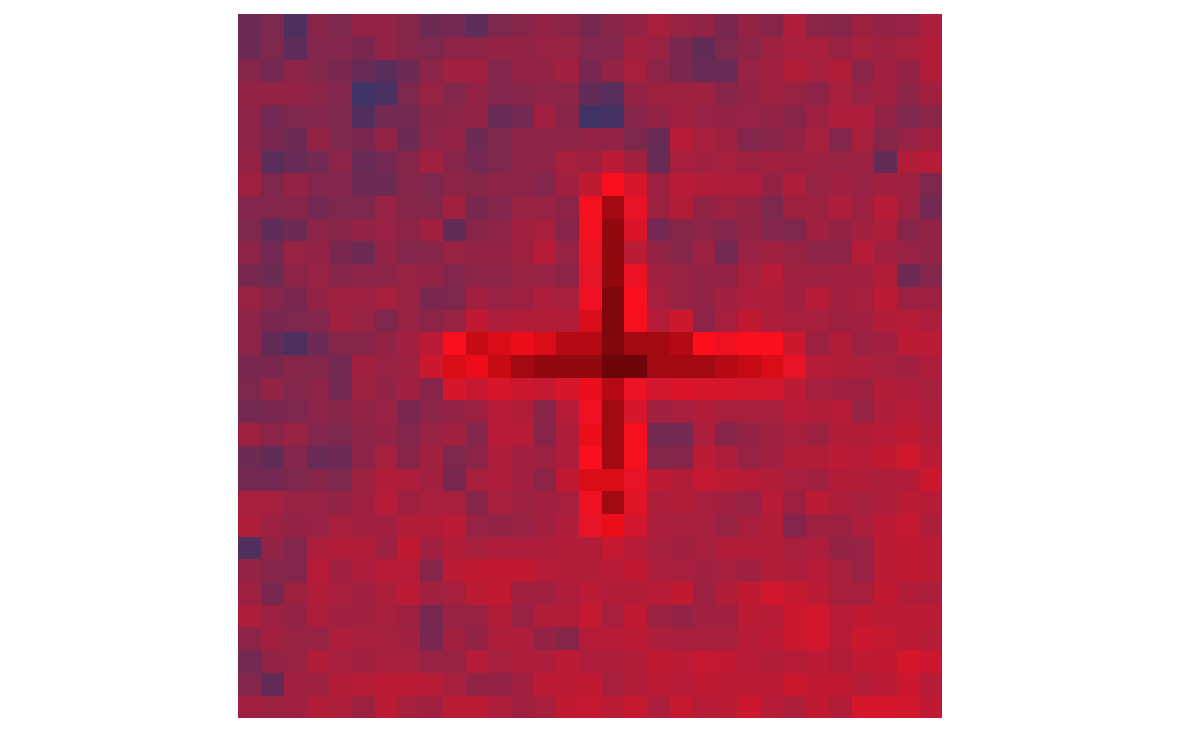
\includegraphics[width=.3\textwidth]{../plots_tables_images/1d1dcrop_6_3.eps}}{\caption{}}%
        \ffigbox[\FBwidth]%
        {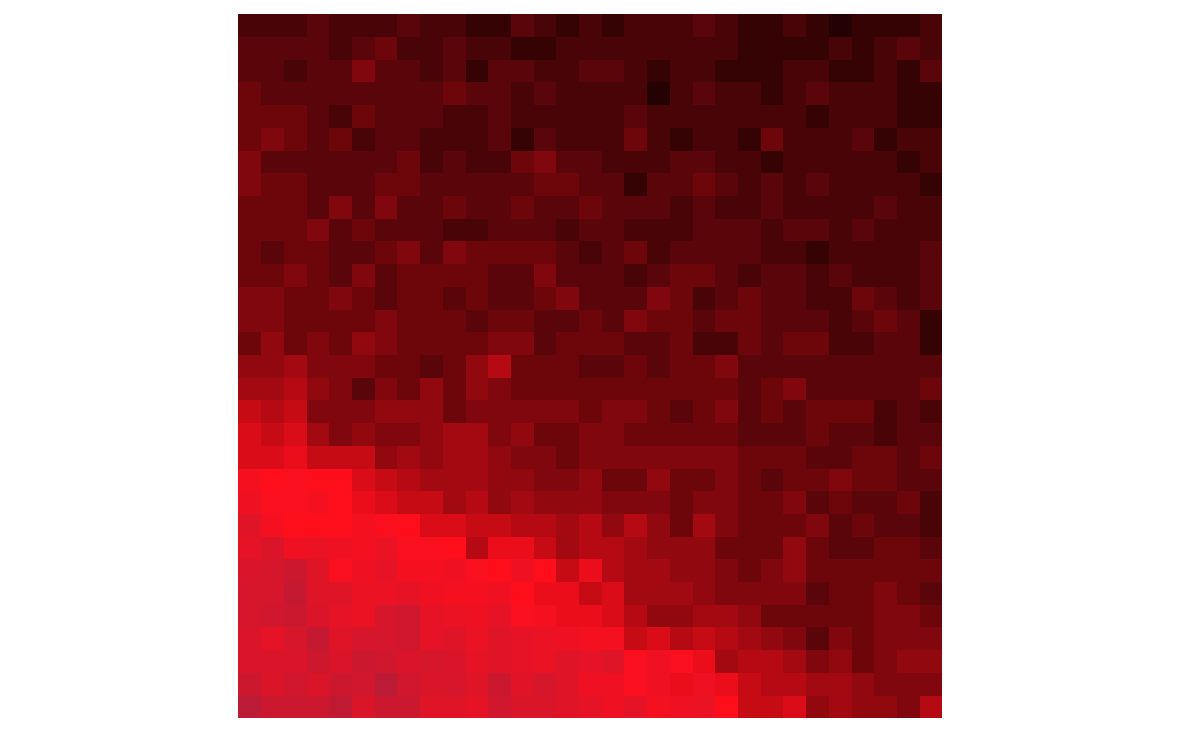
\includegraphics[width=.3\textwidth]{../plots_tables_images/1d1dcrop_6_9.eps}}{\caption{}}%
    \end{subfloatrow}}{\caption{Each possible fiducial candidate}\label{lotsofcrop}} 
\end{figure}

% \begin{figure}[!ht]
%     \vspace{-0.5in}
%     \begin{subfigure}[b]{.3\linewidth}
%         \centering
%         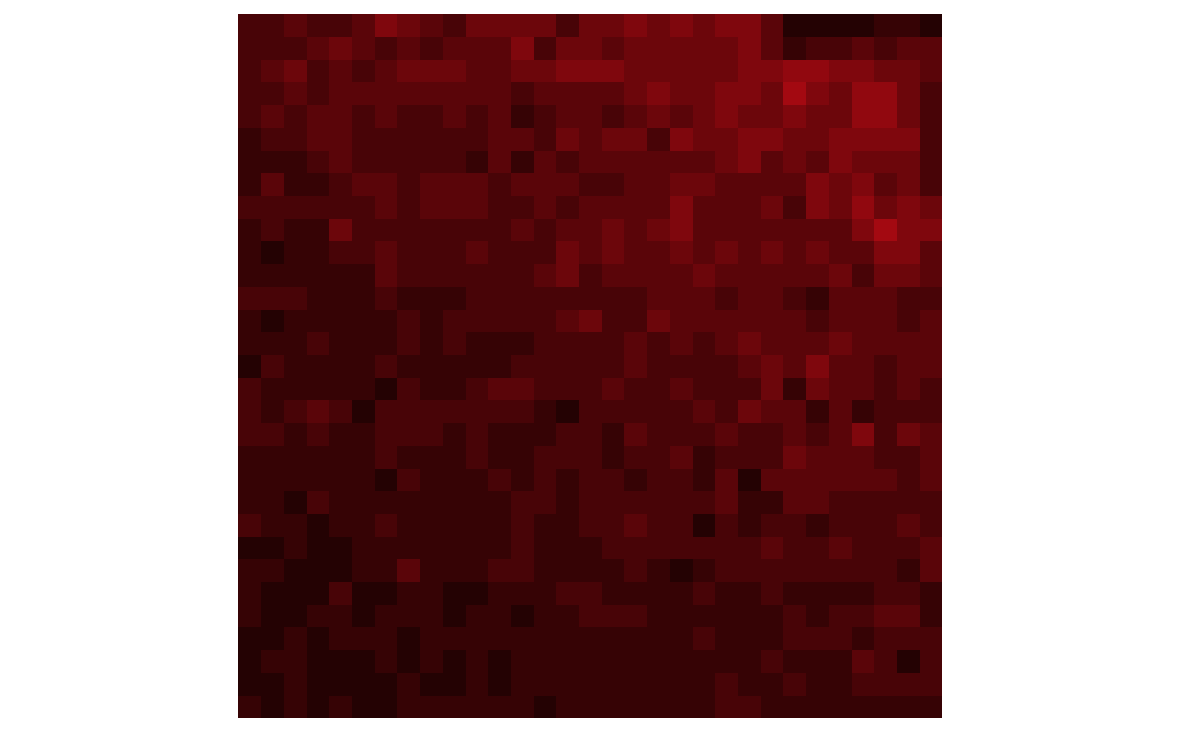
\includegraphics[width=1.2\linewidth]{../plots_tables_images/1d1dcrop_0_0.eps}
%         % \caption{}
%     \end{subfigure}
%     \begin{subfigure}[b]{.3\linewidth}
%         \centering
%         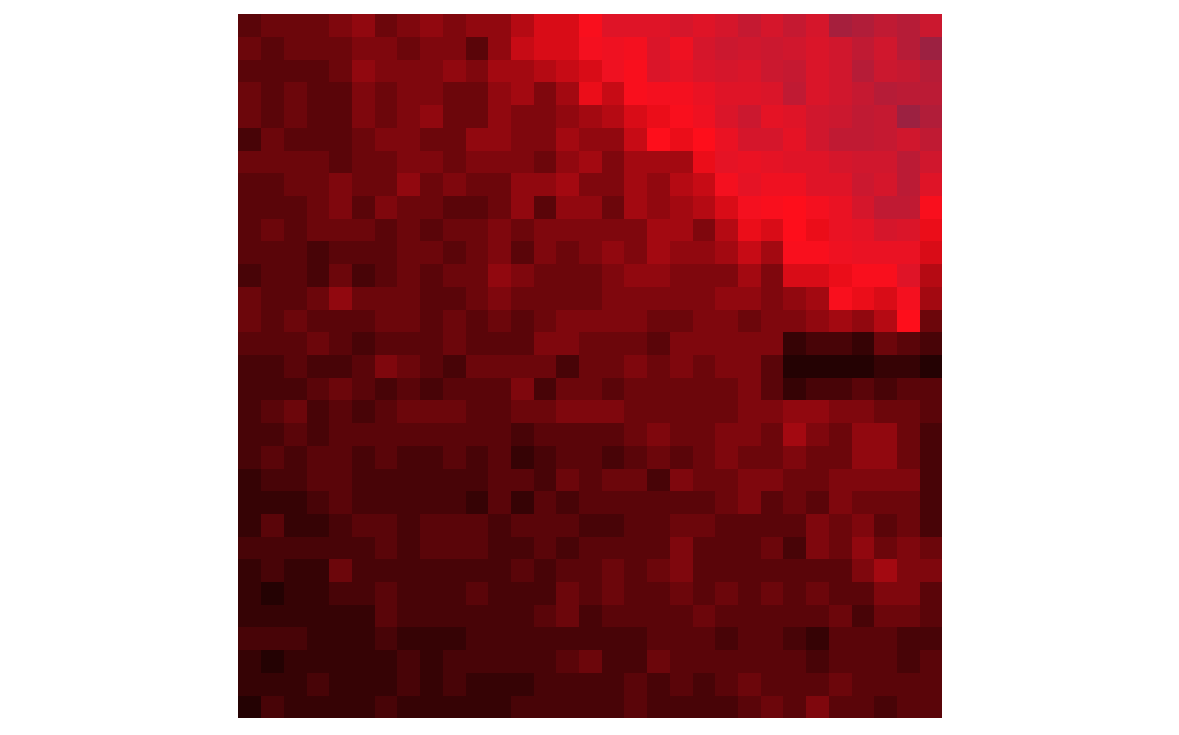
\includegraphics[width=1.2\linewidth]{../plots_tables_images/1d1dcrop_0_1.eps}
%         % \caption{}
%     \end{subfigure}
%     % \hspace{-1.0in}
%     \begin{subfigure}[b]{.3\linewidth}
%         \centering
%         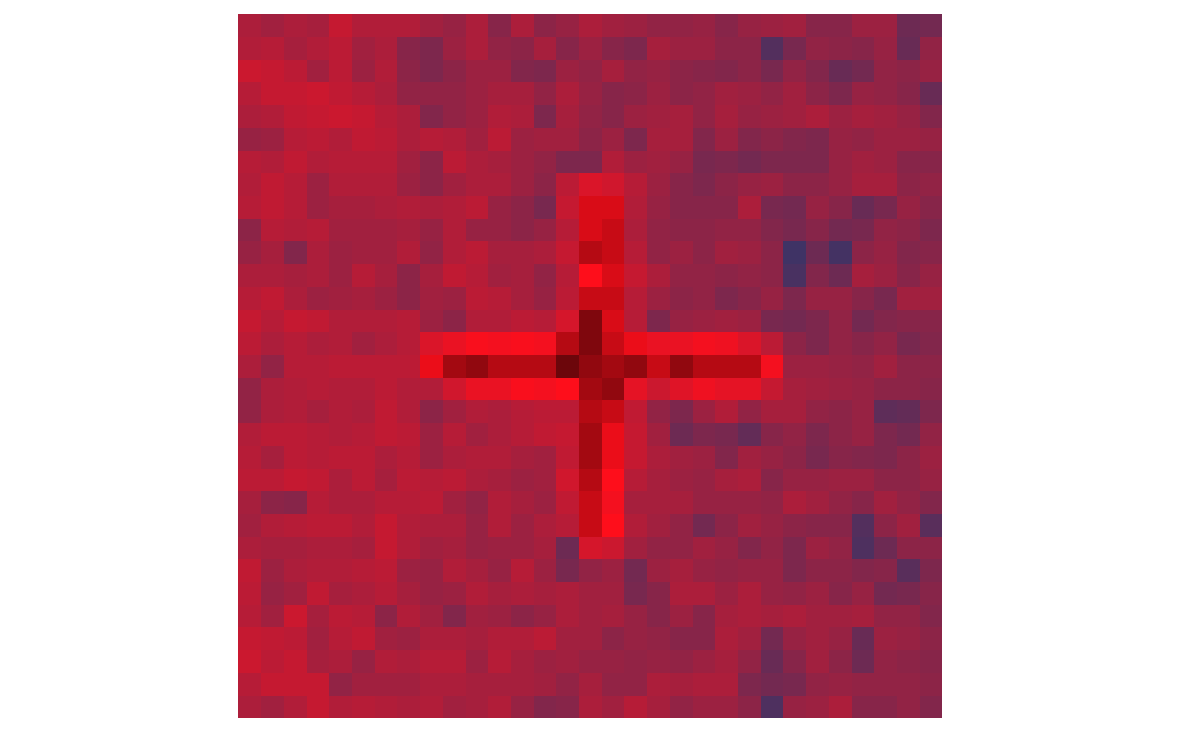
\includegraphics[width=1.2\linewidth]{../plots_tables_images/1d1dcrop_0_4.eps}
%         % \caption{}
%     \end{subfigure}

%     \begin{subfigure}[b]{.3\linewidth}
%         \centering
%         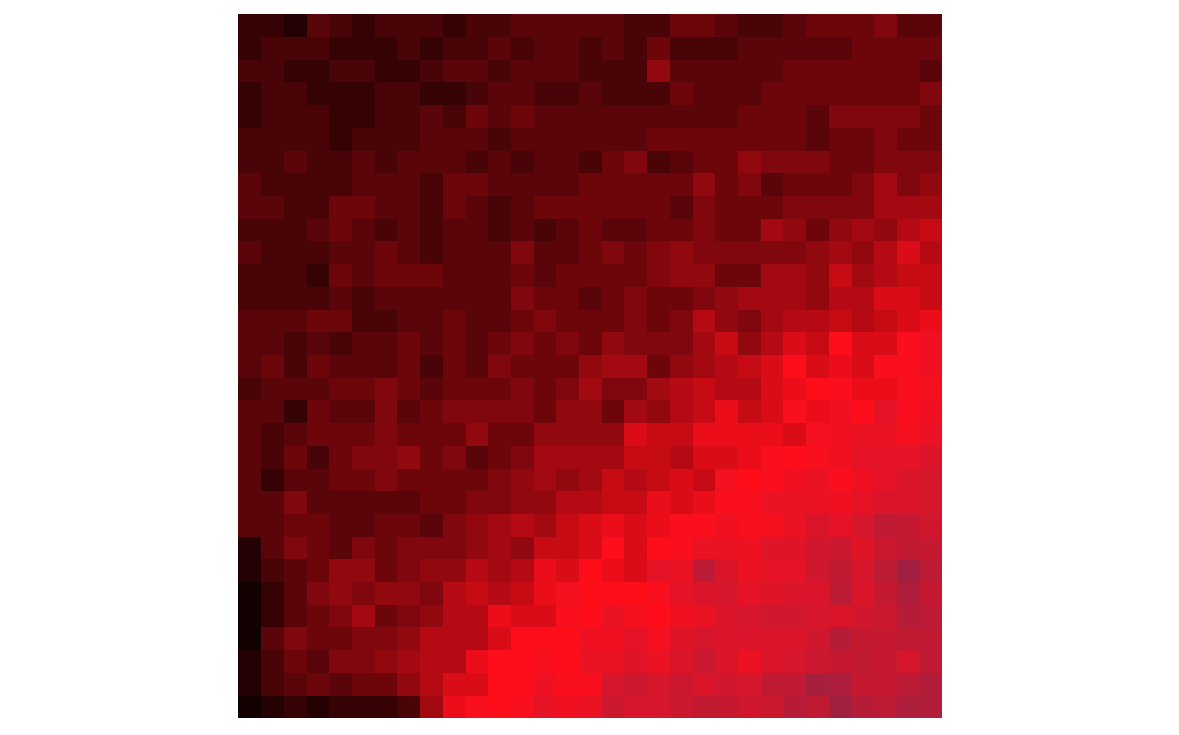
\includegraphics[width=1.2\linewidth]{../plots_tables_images/1d1dcrop_0_8.eps}
%         % \caption{}
%     \end{subfigure}
%     \begin{subfigure}[b]{.3\linewidth}
%         \centering
%         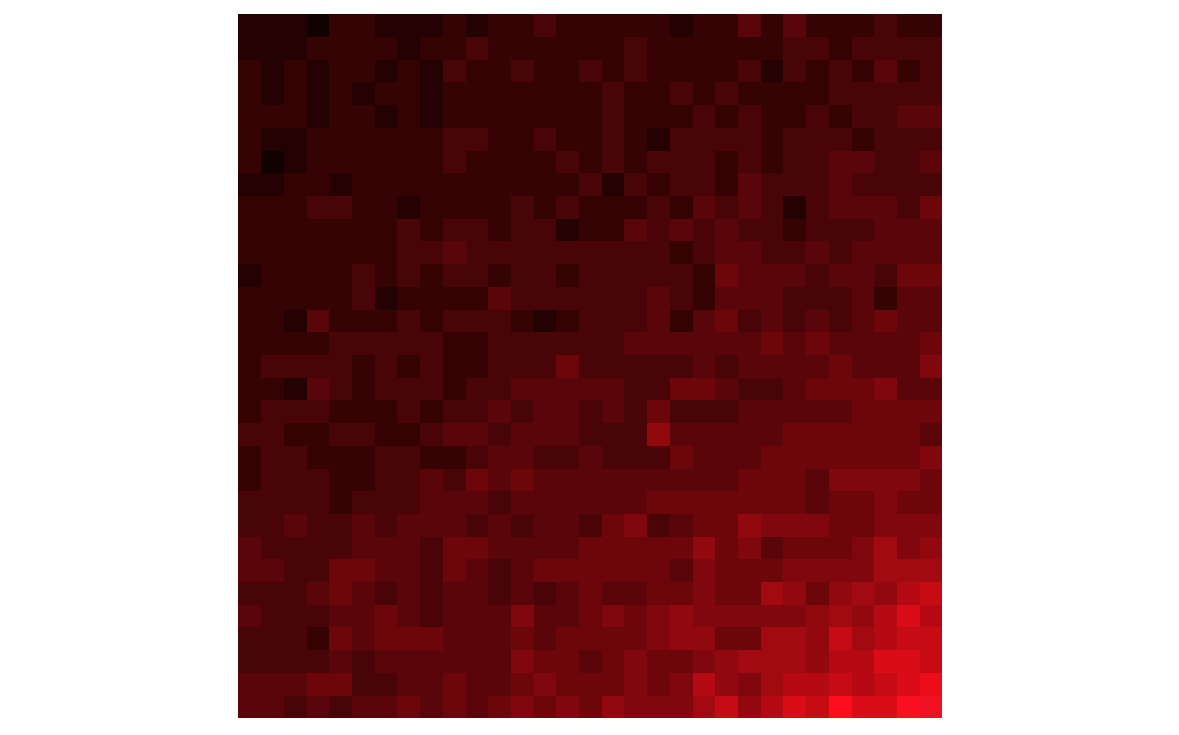
\includegraphics[width=1.2\linewidth]{../plots_tables_images/1d1dcrop_0_9.eps}
%         % \caption{}
%     \end{subfigure}
%     % \hspace{-1.0in}
%     \begin{subfigure}[b]{.3\linewidth}
%         \centering
%         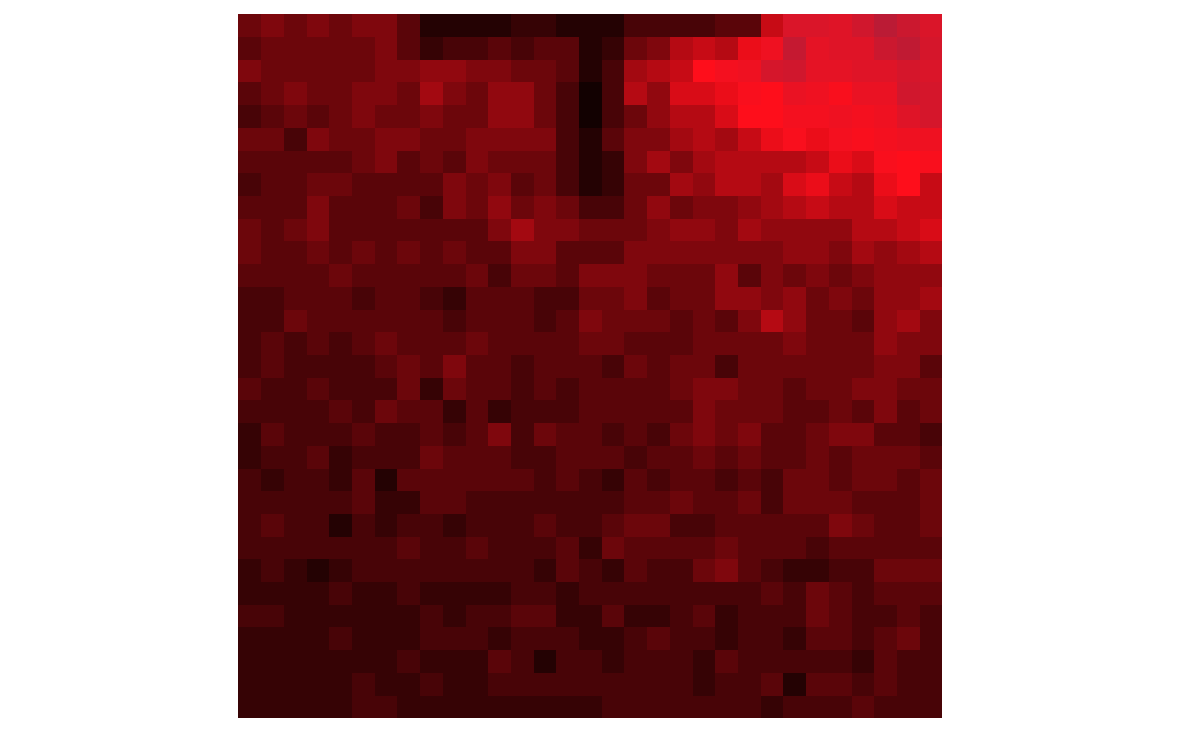
\includegraphics[width=1.2\linewidth]{../plots_tables_images/1d1dcrop_1_0.eps}
%         % \caption{}
%     \end{subfigure}


%     \begin{subfigure}[b]{.3\linewidth}
%         \centering
%         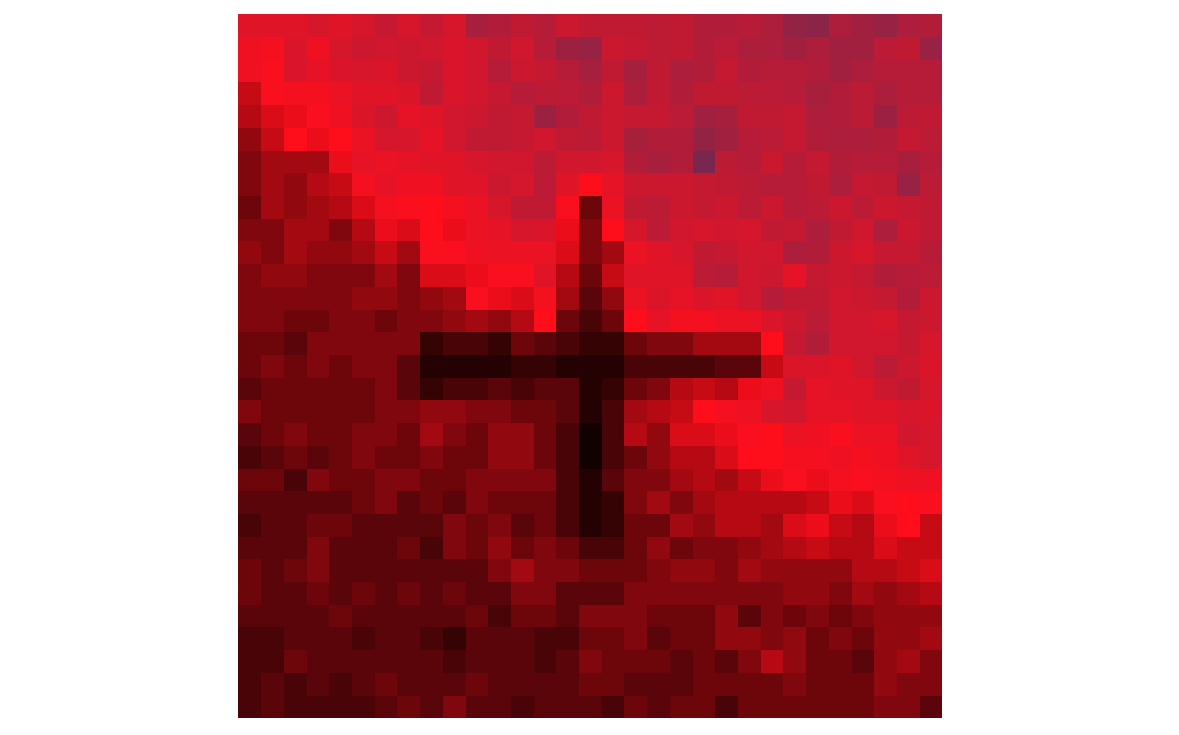
\includegraphics[width=1.2\linewidth]{../plots_tables_images/1d1dcrop_1_1.eps}
%         % \caption{}
%     \end{subfigure}
%     \begin{subfigure}[b]{.3\linewidth}
%         \centering
%         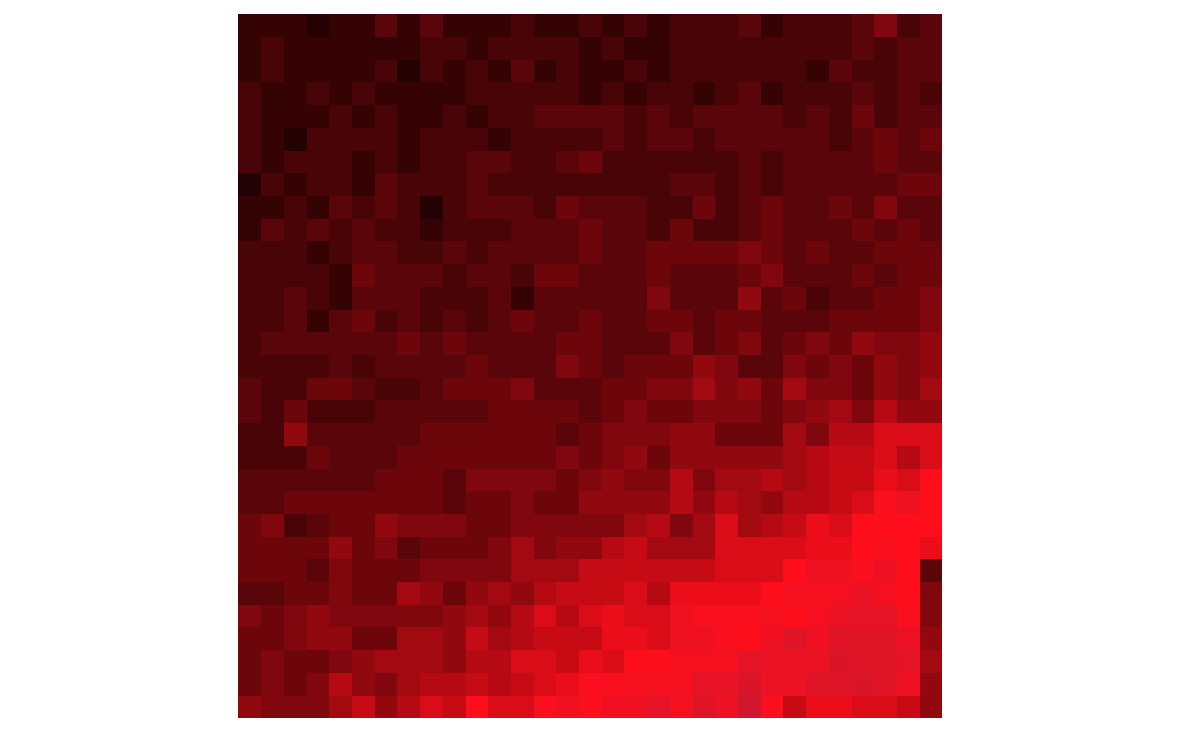
\includegraphics[width=1.2\linewidth]{../plots_tables_images/1d1dcrop_1_9.eps}
%         % \caption{}
%     \end{subfigure}
%     % \hspace{-1.0in}
%     \begin{subfigure}[b]{.3\linewidth}
%         \centering
%         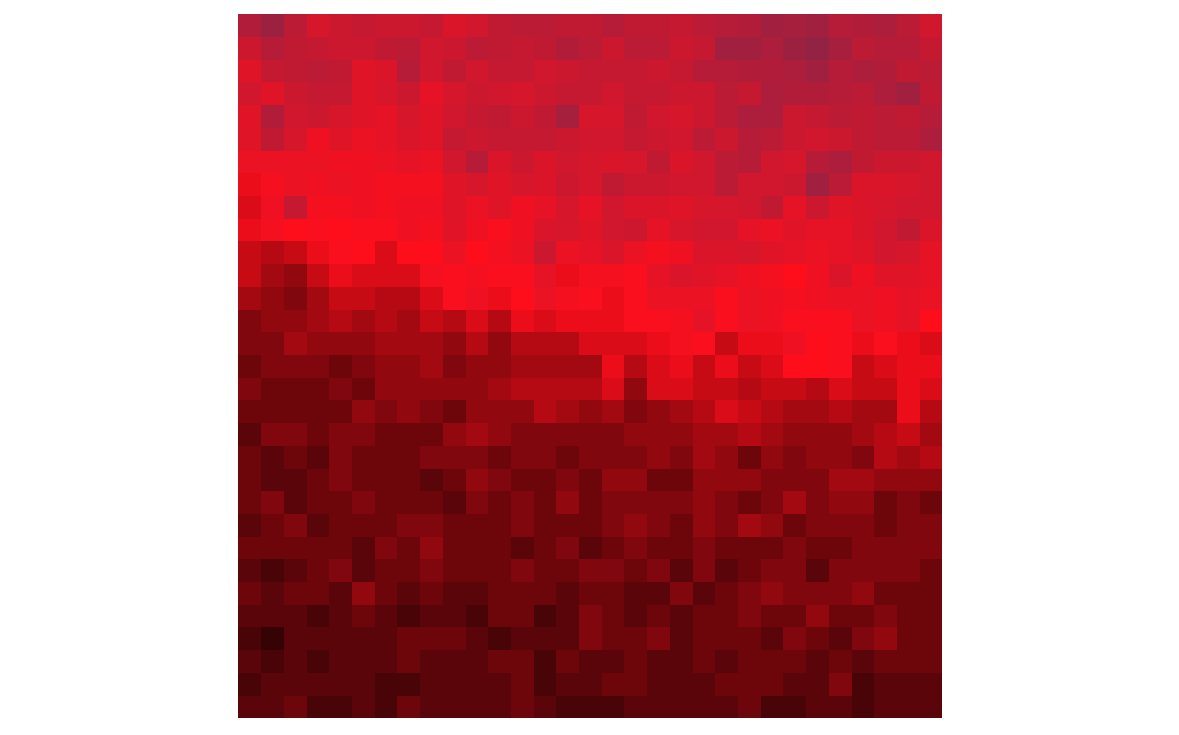
\includegraphics[width=1.2\linewidth]{../plots_tables_images/1d1dcrop_2_0.eps}
%         % \caption{}
%     \end{subfigure}


%     \begin{subfigure}[b]{.3\linewidth}
%         \centering
%         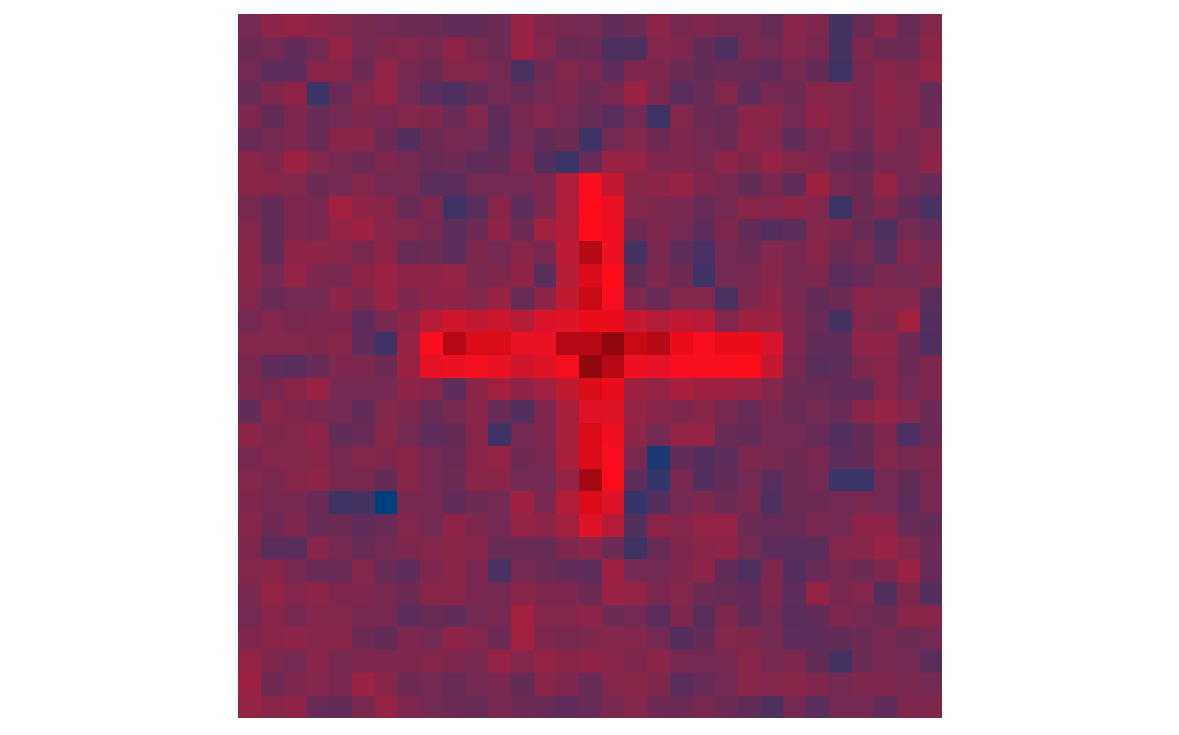
\includegraphics[width=1.2\linewidth]{../plots_tables_images/1d1dcrop_2_5.eps}
%         % \caption{}
%     \end{subfigure}
%     \begin{subfigure}[b]{.3\linewidth}
%         \centering
%         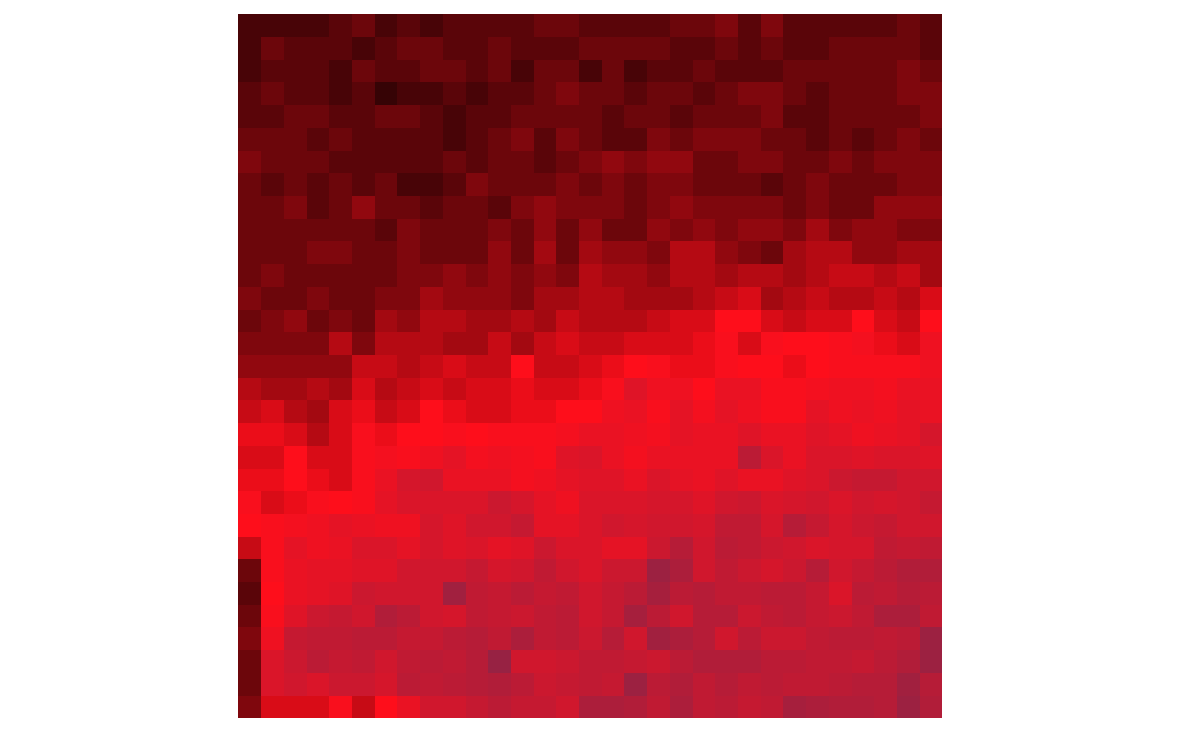
\includegraphics[width=1.2\linewidth]{../plots_tables_images/1d1dcrop_2_9.eps}
%         % \caption{}
%     \end{subfigure}
%     % \hspace{-1.0in}
%     \begin{subfigure}[b]{.3\linewidth}
%         \centering
%         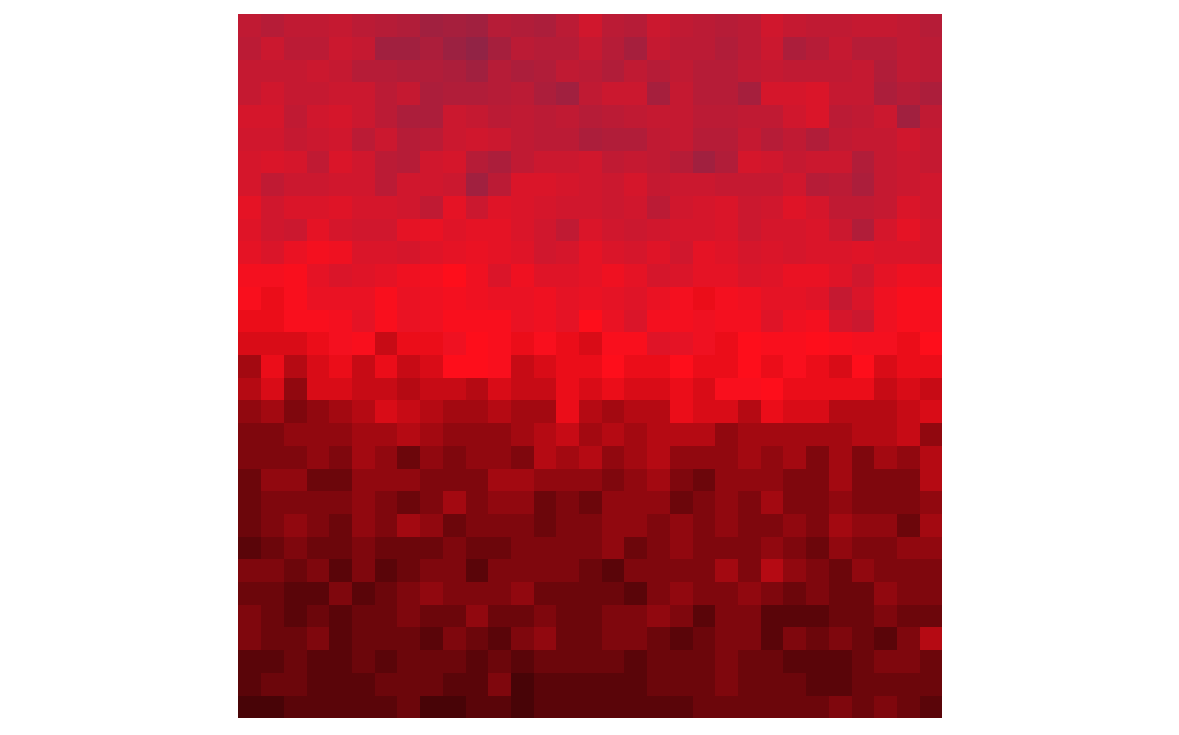
\includegraphics[width=1.2\linewidth]{../plots_tables_images/1d1dcrop_3_0.eps}
%         % \caption{}
%     \end{subfigure}


%     \begin{subfigure}[b]{.3\linewidth}
%         \centering
%         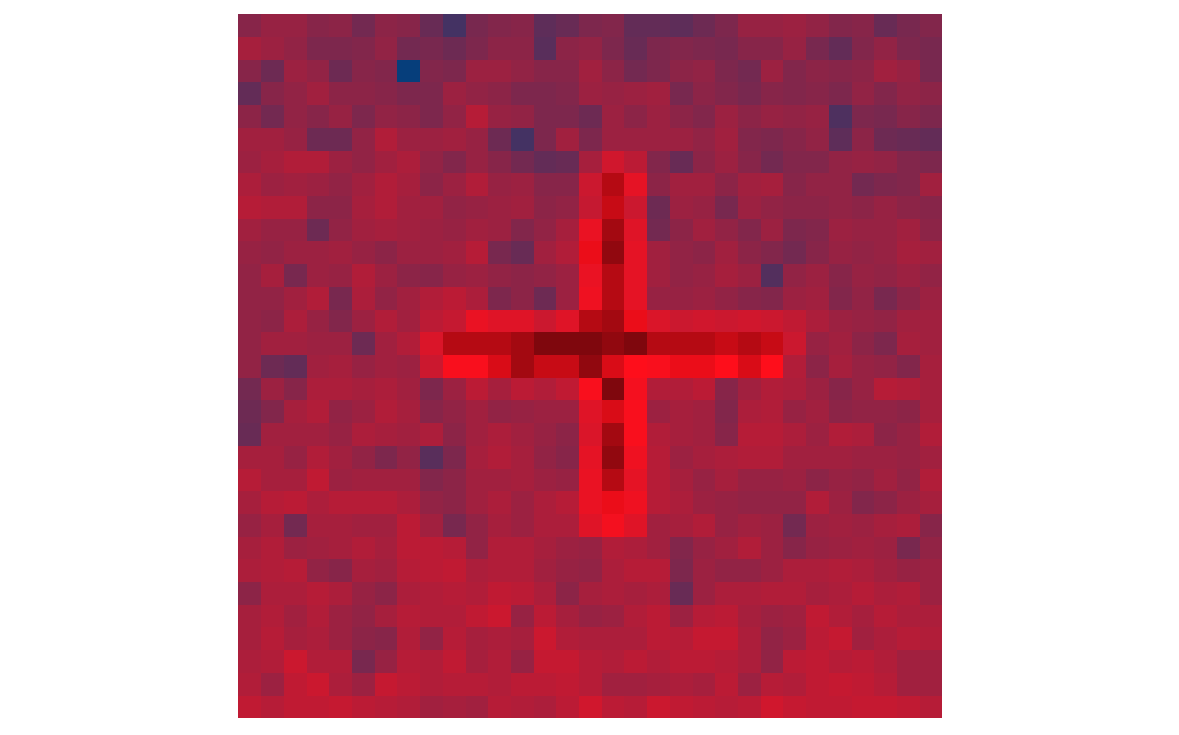
\includegraphics[width=1.2\linewidth]{../plots_tables_images/1d1dcrop_3_2.eps}
%         % \caption{}
%     \end{subfigure}
%     \begin{subfigure}[b]{.3\linewidth}
%         \centering
%         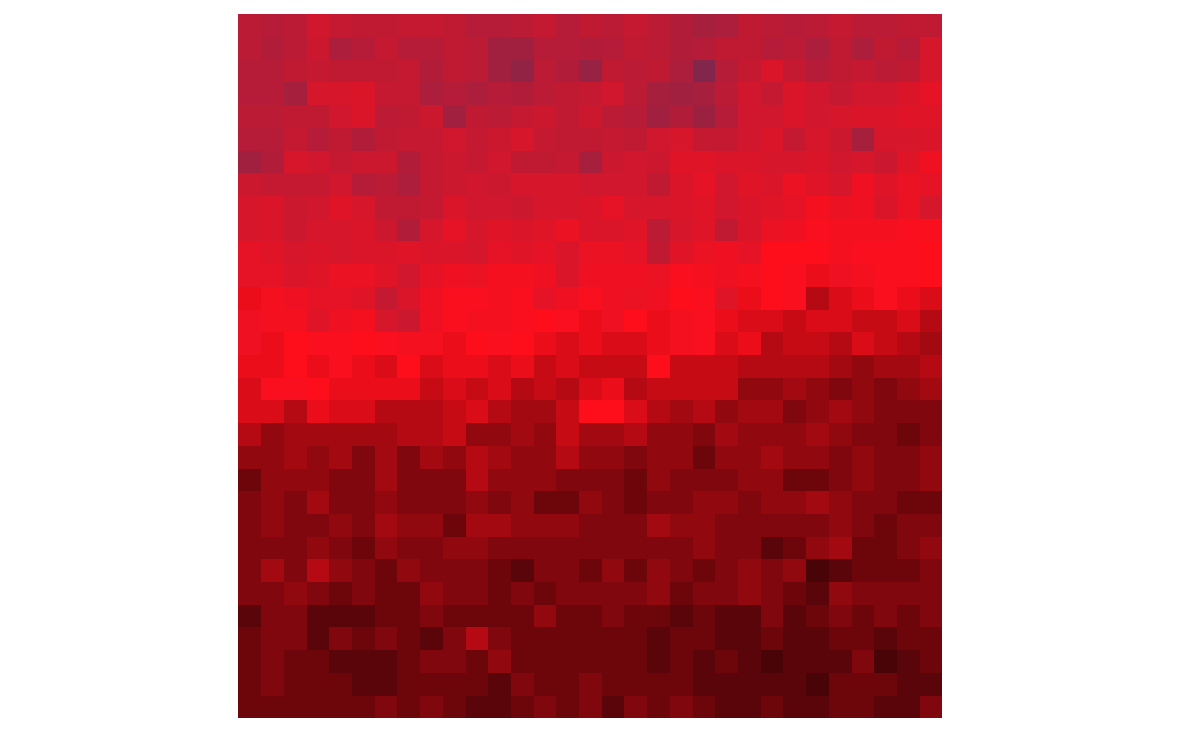
\includegraphics[width=1.2\linewidth]{../plots_tables_images/1d1dcrop_4_0.eps}
%         % \caption{}
%     \end{subfigure}
%     % \hspace{-1.0in}
%     \begin{subfigure}[b]{.3\linewidth}
%         \centering
%         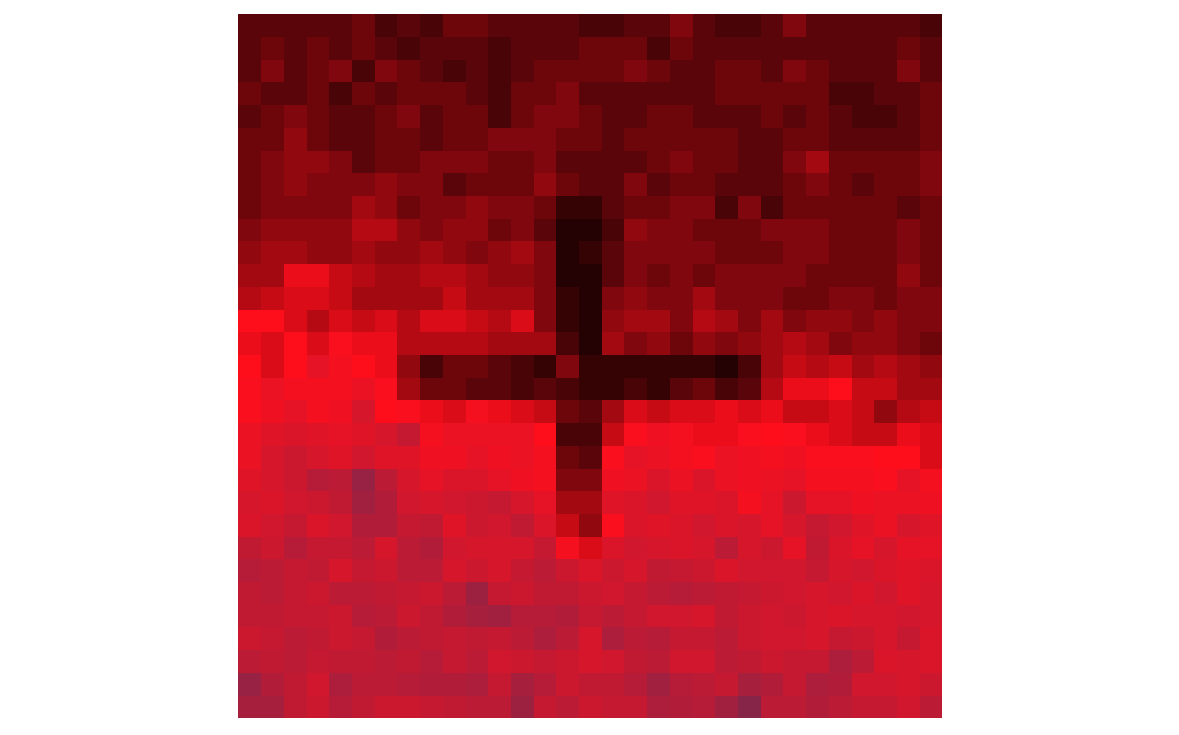
\includegraphics[width=1.2\linewidth]{../plots_tables_images/1d1dcrop_4_9.eps}
%         % \caption{}
%     \end{subfigure}


%     \begin{subfigure}[b]{.3\linewidth}
%         \centering
%         \includegraphics[width=1.2\linewidth]{../plots_tables_images/1d1dcrop_5_0.eps}
%         % \caption{}
%     \end{subfigure}
%     \begin{subfigure}[b]{.3\linewidth}
%         \centering
%         \includegraphics[width=1.2\linewidth]{../plots_tables_images/1d1dcrop_5_6.eps}
%         % \caption{}
%     \end{subfigure}
%     % \hspace{-1.0in}
%     \begin{subfigure}[b]{.3\linewidth}
%         \centering
%         \includegraphics[width=1.2\linewidth]{../plots_tables_images/1d1dcrop_5_9.eps}
%         % \caption{}
%     \end{subfigure}


%     \begin{subfigure}[b]{.3\linewidth}
%         \centering
%         \includegraphics[width=1.2\linewidth]{../plots_tables_images/1d1dcrop_6_0.eps}
%         % \caption{}
%     \end{subfigure}
%     % \hspace{-1.0in}
%     \begin{subfigure}[b]{.3\linewidth}
%         \centering
%         \includegraphics[width=1.2\linewidth]{../plots_tables_images/1d1dcrop_6_3.eps}
%         % \caption{}
%     \end{subfigure}
%     \begin{subfigure}[b]{.3\linewidth}
%         \centering
%         \includegraphics[width=1.2\linewidth]{../plots_tables_images/1d1dcrop_6_9.eps}
%         % \caption{}
%     \end{subfigure}
%     \caption{Each possible fiducial candidate}
%     \label{lotsofcrop}
% \end{figure}


\begin{figure}[!ht]
\vspace{-0.5in}
    \ffigbox[][\FBheight]{%
    \begin{subfloatrow}[3]%
        \ffigbox[\FBwidth]%
        {\includegraphics[width=.3\textwidth]{../plots_tables_images/1d1dsums_0_0.eps}}{}%
        \ffigbox[\FBwidth]%
        {\includegraphics[width=.3\textwidth]{../plots_tables_images/1d1dsums_0_1.eps}}{}%
        \ffigbox[\FBwidth]%
        {\includegraphics[width=.3\textwidth]{../plots_tables_images/1d1dsums_0_4.eps}}{}%
    \end{subfloatrow}}

    \ffigbox[][\FBheight]{%
    \begin{subfloatrow}[3]%
        \ffigbox[\FBwidth]%
        {\includegraphics[width=.3\textwidth]{../plots_tables_images/1d1dsums_0_8.eps}}{}%
        \ffigbox[\FBwidth]%
        {\includegraphics[width=.3\textwidth]{../plots_tables_images/1d1dsums_0_9.eps}}{}%
        \ffigbox[\FBwidth]%
        {\includegraphics[width=.3\textwidth]{../plots_tables_images/1d1dsums_1_0.eps}}{}%
    \end{subfloatrow}}

    \ffigbox[][\FBheight]{%
    \begin{subfloatrow}[3]%
        \ffigbox[\FBwidth]%
        {\includegraphics[width=.3\textwidth]{../plots_tables_images/1d1dsums_1_1.eps}}{}%
        \ffigbox[\FBwidth]%
        {\includegraphics[width=.3\textwidth]{../plots_tables_images/1d1dsums_1_9.eps}}{}%
        \ffigbox[\FBwidth]%
        {\includegraphics[width=.3\textwidth]{../plots_tables_images/1d1dsums_2_0.eps}}{}%
    \end{subfloatrow}}

    \ffigbox[][\FBheight]{%
    \begin{subfloatrow}[3]%
        \ffigbox[\FBwidth]%
        {\includegraphics[width=.3\textwidth]{../plots_tables_images/1d1dsums_2_5.eps}}{}%
        \ffigbox[\FBwidth]%
        {\includegraphics[width=.3\textwidth]{../plots_tables_images/1d1dsums_2_9.eps}}{}%
        \ffigbox[\FBwidth]%
        {\includegraphics[width=.3\textwidth]{../plots_tables_images/1d1dsums_3_0.eps}}{}%
    \end{subfloatrow}}

    \ffigbox[][\FBheight]{%
    \begin{subfloatrow}[3]%
        \ffigbox[\FBwidth]%
        {\includegraphics[width=.3\textwidth]{../plots_tables_images/1d1dsums_3_2.eps}}{}%
        \ffigbox[\FBwidth]%
        {\includegraphics[width=.3\textwidth]{../plots_tables_images/1d1dsums_4_0.eps}}{}%
        \ffigbox[\FBwidth]%
        {\includegraphics[width=.3\textwidth]{../plots_tables_images/1d1dsums_4_9.eps}}{}%
    \end{subfloatrow}}

    \ffigbox[][\FBheight]{%
    \begin{subfloatrow}[3]%
        \ffigbox[\FBwidth]%
        {\includegraphics[width=.3\textwidth]{../plots_tables_images/1d1dsums_5_0.eps}}{}%
        \ffigbox[\FBwidth]%
        {\includegraphics[width=.3\textwidth]{../plots_tables_images/1d1dsums_5_6.eps}}{}%
        \ffigbox[\FBwidth]%
        {\includegraphics[width=.3\textwidth]{../plots_tables_images/1d1dsums_5_9.eps}}{}%
    \end{subfloatrow}}

    \ffigbox[][\FBheight]{%
    \begin{subfloatrow}[3]%
        \ffigbox[\FBwidth]%
        {\includegraphics[width=.3\textwidth]{../plots_tables_images/1d1dsums_6_0.eps}}{\caption{}}%
        \ffigbox[\FBwidth]%
        {\includegraphics[width=.3\textwidth]{../plots_tables_images/1d1dsums_6_3.eps}}{\caption{}}%
        \ffigbox[\FBwidth]%
        {\includegraphics[width=.3\textwidth]{../plots_tables_images/1d1dsums_6_9.eps}}{\caption{}}%
    \end{subfloatrow}}{\caption{The position of the plots above corresponds to the same regions in Figure \ref{lotsofcrop}. The horizontal line is at 100; if there are any elements of the array above 100 for both a column 1D sum and a row 1D sum, then the cropped area is considered to have a fiducial in it. A parabolic fit is applied to 3 consecutive pixels with the center pixel at the peak of the array.}\label{lotsofplot}} 
\end{figure}


% \begin{figure}[!ht]
%     \vspace{-0.5in}
%     \begin{subfigure}[b]{.3\linewidth}
%         \centering
%         \includegraphics[width=1.0\linewidth]{../plots_tables_images/1d1dsums_0_0.eps}
%         % \caption{}
%     \end{subfigure}
%     \begin{subfigure}[b]{.3\linewidth}
%         \centering
%         \includegraphics[width=1.0\linewidth]{../plots_tables_images/1d1dsums_0_1.eps}
%         % \caption{}
%     \end{subfigure}
%     % \hspace{-1.0in}
%     \begin{subfigure}[b]{.3\linewidth}
%         \centering
%         \includegraphics[width=1.0\linewidth]{../plots_tables_images/1d1dsums_0_4.eps}
%         % \caption{}
%     \end{subfigure}
% \vspace{0.2in}

%     \begin{subfigure}[b]{.3\linewidth}
%         \centering
%         \includegraphics[width=1.0\linewidth]{../plots_tables_images/1d1dsums_0_8.eps}
%         % \caption{}
%     \end{subfigure}
%     \begin{subfigure}[b]{.3\linewidth}
%         \centering
%         \includegraphics[width=1.0\linewidth]{../plots_tables_images/1d1dsums_0_9.eps}
%         % \caption{}
%     \end{subfigure}
%     % \hspace{-1.0in}
%     \begin{subfigure}[b]{.3\linewidth}
%         \centering
%         \includegraphics[width=1.0\linewidth]{../plots_tables_images/1d1dsums_1_0.eps}
%         % \caption{}
%     \end{subfigure}
% \vspace{0.2in}

%     \begin{subfigure}[b]{.3\linewidth}
%         \centering
%         \includegraphics[width=1.0\linewidth]{../plots_tables_images/1d1dsums_1_1.eps}
%         % \caption{}
%     \end{subfigure}
%     \begin{subfigure}[b]{.3\linewidth}
%         \centering
%         \includegraphics[width=1.0\linewidth]{../plots_tables_images/1d1dsums_1_9.eps}
%         % \caption{}
%     \end{subfigure}
%     % \hspace{-1.0in}
%     \begin{subfigure}[b]{.3\linewidth}
%         \centering
%         \includegraphics[width=1.0\linewidth]{../plots_tables_images/1d1dsums_2_0.eps}
%         % \caption{}
%     \end{subfigure}
% \vspace{0.2in}

%     \begin{subfigure}[b]{.3\linewidth}
%         \centering
%         \includegraphics[width=1.0\linewidth]{../plots_tables_images/1d1dsums_2_5.eps}
%         % \caption{}
%     \end{subfigure}
%     \begin{subfigure}[b]{.3\linewidth}
%         \centering
%         \includegraphics[width=1.0\linewidth]{../plots_tables_images/1d1dsums_2_9.eps}
%         % \caption{}
%     \end{subfigure}
%     % \hspace{-1.0in}
%     \begin{subfigure}[b]{.3\linewidth}
%         \centering
%         \includegraphics[width=1.0\linewidth]{../plots_tables_images/1d1dsums_3_0.eps}
%         % \caption{}
%     \end{subfigure}
% \vspace{0.2in}

%     \begin{subfigure}[b]{.3\linewidth}
%         \centering
%         \includegraphics[width=1.0\linewidth]{../plots_tables_images/1d1dsums_3_2.eps}
%         % \caption{}
%     \end{subfigure}
%     \begin{subfigure}[b]{.3\linewidth}
%         \centering
%         \includegraphics[width=1.0\linewidth]{../plots_tables_images/1d1dsums_4_0.eps}
%         % \caption{}
%     \end{subfigure}
%     % \hspace{-1.0in}
%     \begin{subfigure}[b]{.3\linewidth}
%         \centering
%         \includegraphics[width=1.0\linewidth]{../plots_tables_images/1d1dsums_4_9.eps}
%         % \caption{}
%     \end{subfigure}
% \vspace{0.2in}

%     \begin{subfigure}[b]{.3\linewidth}
%         \centering
%         \includegraphics[width=1.0\linewidth]{../plots_tables_images/1d1dsums_5_0.eps}
%         % \caption{}
%     \end{subfigure}
%     \begin{subfigure}[b]{.3\linewidth}
%         \centering
%         \includegraphics[width=1.0\linewidth]{../plots_tables_images/1d1dsums_5_6.eps}
%         % \caption{}
%     \end{subfigure}
%     % \hspace{-1.0in}
%     \begin{subfigure}[b]{.3\linewidth}
%         \centering
%         \includegraphics[width=1.0\linewidth]{../plots_tables_images/1d1dsums_5_9.eps}
%         % \caption{}
%     \end{subfigure}
% \vspace{0.2in}

%     \begin{subfigure}[b]{.3\linewidth}
%         \centering
%         \includegraphics[width=1.0\linewidth]{../plots_tables_images/1d1dsums_6_0.eps}
%         % \caption{}
%     \end{subfigure}
%     % \hspace{-1.0in}
%     \begin{subfigure}[b]{.3\linewidth}
%         \centering
%         \includegraphics[width=1.0\linewidth]{../plots_tables_images/1d1dsums_6_3.eps}
%         % \caption{}
%     \end{subfigure}
%     \begin{subfigure}[b]{.3\linewidth}
%         \centering
%         \includegraphics[width=1.0\linewidth]{../plots_tables_images/1d1dsums_6_9.eps}
%         % \caption{}
%     \end{subfigure}
%     \caption{The position of the plots above corresponds to the same regions in Figure \ref{lotsofcrop}. The horizontal line is at 100; if there are any elements of the array above 100 for both a column 1D sum and a row 1D sum, then the cropped area is considered to have a fiducial in it. A parabolic fit is applied to 3 consecutive pixels with the center pixel at the peak of the array.}
%     \label{lotsofplot}
% \end{figure}

\subsection{How Robust is Fiducial Finding?} % (fold)
\label{sub:how_robust_is_fiducial_finding_}
    We wanted to see how our program fared when working on our smaller (449x320) original image.With the same approach, we wanted to see if the 1D sum method would return enough fiducials to accurately orient our image. For reference, the original starting image is shown in Figure \ref{orig}. 

\begin{figure}[!ht]
    \ffigbox[][\FBheight]{%
    \begin{subfloatrow}[2]%
        \ffigbox[\FBwidth]%
       {%
       \includegraphics[width=.5\textwidth]{../plots_tables_images/orig_sun.jpg}%
       }%
       {%
       \caption{}%
       \label{orig}%
       }%
        \ffigbox[\Xhsize]%
       {%
       \includegraphics[width=.5\textwidth]{../plots_tables_images/smooth_fid_test.eps}%
       }%
       {%
       \caption{Fiducial positions returned by 1D sum method on smaller, blurrier image. Ignore the bright pixel next to the bottom left fiducial.}%
       \label{smoothed_fid_test}%
       }%
    \end{subfloatrow}}{\caption{}}%
\end{figure}

% \begin{figure}[!ht]
%     \begin{subfigure}[b]{.5\linewidth}
%         \centering
%         \includegraphics[width=\linewidth]{../plots_tables_images/orig_sun.jpg}
%         \caption{}
%         \label{orig}
%     \end{subfigure}
%     \begin{subfigure}[b]{.5\linewidth}
%         \centering
%         \includegraphics[width=\linewidth]{../plots_tables_images/smooth_fid_test.eps}
%         \caption{Fiducial positions returned by 1D sum method on smaller, blurrier image. Ignore the bright pixel next to the bottom left fiducial.}
%         \label{smoothed_fid_test}
%     \end{subfigure}
%     \caption{}
% \end{figure}


There was a problem with the lack of pixels which resulted in the \hl{\texttt{array - smooth(array,n\_smooth)}} plot to have peaks in the wrong places. To address this, we set an arbitrary threshold at 1000 and only smoothed pixels with higher values. Illustrated in Figure \ref{fix_small}, this method has the potential to ignore fiducials on the very limbs of the sun, but if that is the case, then the first set of 1D sums across the entire sun would likely not pick up the faint dip in the 1D sum and would thus not even think to look there. \\
\indent Figure \ref{smoothed_fid_test} shows how our code fares when finding the fiducials of an image that is significantly smaller than our Albert-approved image.

\begin{figure}[!ht]
    \ffigbox[][\FBheight]{%
    \begin{subfloatrow}[2]%
        \ffigbox[\FBwidth]%
       {%
       \includegraphics[width=.5\textwidth]{../plots_tables_images/small_image.eps}%
       }%
       {%
       \caption{In the top set of plots, the solid line is the 1D sum, the dotted line is the 1D sum smoothed by 5 pixels. In the bottom set of plots, the difference of the 1D sum and the smoothed 1D sum is shown. Notice the small dip at index 10 which is dominated by the smoothing artifact of the limb at indices 0 to 5.}%
       \label{small_image}%
       }%
        \ffigbox[\Xhsize]%
       {%
       \includegraphics[width=.5\textwidth]{../plots_tables_images/small_image_fixed.eps}%
       }%
       {%
       \caption{The 1D sum is thresholded to be only above 1000 and the process is repeated, this time the difference in the two arrays returns a clear peak.}%
       \label{small_image_fixed}%
       }%
    \end{subfloatrow}}{\caption{}\label{fix_small}}%
\end{figure}

% \begin{figure}[!ht]
%     \begin{subfigure}[b]{.5\linewidth}
%         \centering
%         \includegraphics[width=\linewidth]{../plots_tables_images/small_image.eps}
%         \caption{In the top set of plots, the solid line is the 1D sum, the dotted line is the 1D sum smoothed by 5 pixels. In the bottom set of plots, the difference of the 1D sum and the smoothed 1D sum is shown. Notice the small dip at index 10 which is dominated by the smoothing artifact of the limb at indices 0 to 5.}
%         \label{small_image}
%     \end{subfigure}
%     \begin{subfigure}[b]{.5\linewidth}
%         \centering
%         \includegraphics[width=\linewidth]{../plots_tables_images/small_image_fixed.eps}
%         \caption{The 1D sum is thresholded to be only above 1000 and the process is repeated, this time the difference in the two arrays returns a clear peak.}
%         \label{small_image_fixed}
%     \end{subfigure}
%     \caption{}
%     \label{fix_small}
% \end{figure}

% subsection how_robust_is_fiducial_finding_ (end)


% section finding_fiducials (end)


\end{document}










